\documentclass[12pt,a4paper,hidelinks]{report}
\usepackage{amsmath,amsthm,amssymb,graphicx,hyperref,mathptmx}
\usepackage[left=1.2in,right=1in,top=1in,bottom=1in]{geometry}
\usepackage[romanian]{babel}
\usepackage{float}
\usepackage{listings}
\usepackage{color}
\definecolor{dkgreen}{rgb}{0,0.6,0}
\definecolor{gray}{rgb}{0.5,0.5,0.5}
\definecolor{mauve}{rgb}{0.58,0,0.82}
%\usepackage{...insert other packages here...}
\newtheorem{thm}{Teorema}[section]
\newtheorem{lem}[thm]{Lema}
\newtheorem{cor}[thm]{Corolarul}
\newtheorem{prop}[thm]{Propozi\c tia}
\theoremstyle{definition}
\newtheorem{defn}{Defini\c tia}[section]
\theoremstyle{remark}
\newtheorem{rem}{Remarca}[section]
\newtheorem{exmp}{Exemplul}[section]
\begin{document}
\thispagestyle{empty}
\begin{center}
\begin{figure}[h!]
\vspace{-20pt}
\begin{center}

\includegraphics[width=100pt]{images/FMI-03.png}
\end{center}
\end{figure}
\lstdefinelanguage{JavaScript}{
  keywords={typeof, new, true, false, catch, function, return, null, catch, switch, var, if, in, while, do, else, case, break},
  keywordstyle=\color{dkgreen}\bfseries,
  ndkeywords={class, export, boolean, throw, implements, import, this, async},
  ndkeywordstyle=\color{gray}\bfseries,
  identifierstyle=\color{black},
  sensitive=false,
  comment=[l]{//},
  morecomment=[s]{/*}{*/},
  commentstyle=\color{dkgreen}\ttfamily,
  stringstyle=\color{mauve}\ttfamily,
  morestring=[b]',
  morestring=[b]"
}
\lstset{frame=tb,
    language=JavaScript,
    aboveskip=5mm, belowskip=3mm, showstringspaces=false,
    columns=flexible, basicstyle={\small\ttfamily},
    numbers=none, numberstyle=\tiny\color{gray},
    keywordstyle=\color{blue},
    commentstyle=\color{dkgreen},
    stringstyle=\color{mauve},
    breaklines=true,
    breakatwhitespace=true,
    tabsize=1,
    basicstyle={\scriptsize\ttfamily}
}


{\large{\bf UNIVERSITATEA DE VEST DIN TIMI\c SOARA

FACULTATEA DE MATEMATIC\u A \c SI INFORMATIC\u A

PROGRAMUL DE STUDII DE LICEN\c T\u A: INFORMATIC\u A APLICAT\u A}}

\vspace{120pt}
{\huge {\bf LUCRARE DE LICEN\c T\u A}}

\vspace{150pt}
\end{center}

{\large\noindent{\bf COORDONATOR:\hfill ABSOLVENT:}

\noindent Conf. Dr. Forti\c s Florin \hfill Vidican Vlad-George}

\vfill
\begin{center}
{\bf TIMI\c SOARA

2023}
\end{center}
\newpage
\thispagestyle{empty}
\begin{center}
{\large{\bf UNIVERSITATEA DE VEST DIN TIMI\c SOARA

FACULTATEA DE MATEMATIC\u A \c SI INFORMATIC\u A

PROGRAMUL DE STUDII DE LICEN\c T\u A: INFORMATIC\u A APLICAT\u A}}

\vspace{120pt}
%{\huge {\bf LUCRARE DE LICEN\c T\u A/DIZERTA\c TIE}}
{\huge {\bf ThesisHub: Platforma web pentru lucr\u ari de licen\c t\u a/Dizerta\c tie}}

\vspace{150pt}
\end{center}

{\large\noindent{\bf COORDONATOR:\hfill ABSOLVENT:}

\noindent Conf. Dr. Forti\c s Florin \hfill Vidican Vlad-George}

\vfill
\begin{center}
{\bf TIMI\c SOARA23

2023}
\end{center}
\newpage
\normalsize{}
\tableofcontents
\newpage
\chapter{Introducere}
\addcontentsline{toc}{chapter}{Introducere}

\section{Descrierea problemei}
Tema aleasă de către mine constă în dezvoltarea unei platforme online destinată studenților în anii terminali la unul dintre ciclurile de învățământ superior și profesorilor universitari în scopul coordonări sau găsirii unui coordonator pentru elaborarea lucrării de licența sau dizertație. Principalul mod în care platforma în cauză își propune să ajute în această privința este prin a facilita comunicarea dintre studenți și profesori, utilizatorii având posibilitatea de a-și posta propriile propuneri de teme sau de a aplica pentru unele din cele disponibile si active în acel moment, reducând astfel potențialul timp mort apărut pentru student în momentul aplicării pentru propuneri de teme a căror disponibilitate nu le este încă cunoscută dar și reducând comunicarea redundantă de ambele parți, propunerile având o secțiune de comentarii unde se pot acoperi eventualele întrebări frecvente.
\chapter{Solutii Similare}
\addcontentsline{toc}{chapter}{Solutii similare}
\section{Servicii de consultanta}
\subsection{Gradcoach}
\textbf{\textit{Gradcoach}} \footnote[1]{https://gradcoach.com/services/} este o platformă online care oferă suport contra cost studenților în realizarea lucrării de licența/dizertație, suportul variază în funcție de planul ales putând presupune:
\begin{itemize}
    \item Consiliere one-on-one cu un mentor specialist în domeniul temei alese. În timpul întâlnirii se pot discută: progresul, eventuale puncte de blocare și sugestii de îmbunătățire.
    \item Crearea și distribuirea de chestionare. colectarea și compilarea acestor răspunsuri. Transcripție în cazul în care datele colectate vin în format audio sau audio-video și codarea datelor.
    \item Ajustări pentru variantă finală a lucrării, cum ar fi repararea greșelilor gramaticale, asigurarea consecvenței și respectării standardelor universității în ceea ce privește redactarea lucrării (font, spațiere, cuprins, citate și referințe, numerotarea paginii).
\end{itemize}




\subsection{ThesisHelpers}
\textbf{\textit{Thesishelpers}}\footnote[2]{https://www.thesishelpers.com/about} este o platformă online similară cu gradcoach, în sensul că și aceasta oferă servicii studenților pentru realizarea lucrării de licența/dizertație, aceste servici fiind: 
\begin{itemize}
    \item Ajustări pentru varianta finală a lucrării.
    \item Editare ușoara (restructurarea textului, rescrierea anumitor propoziții pentru o alegere mai bună a cuvintelor păstrând însă ideea din spate intactă).
    \item Realizarea întregi lucrări, clientul fiind responsabil doar de setarea cerințelor pentru această lucrare.
\end{itemize} 
\subsection{Compara\c tie}
Soluția mea este diferită față de cele două platforme menționate mai sus, deoarece aceasta va fi o platformă internă, non-profit care își propune doar să faciliteze comunicarea dintre studenți și profesori în scopul realizării lucrării necesare pentru absolvirea ciclului de studiu ales în timp ce platformele menționate mai sus oferă servicii contra cost a unor consultanți externi, unele dintre aceste servicii presupunând chiar plagiarism și implicit încălcarea integrității academice
\section{Platforme de matchmaking}
O platformă de matchmaking are ca scop fundamental potrivirea de persoane. Matchmaking-ul este un termen-umbrelă destul de vast, care acoperă o multitudine de servicii/platforme, toate aceste servicii având însă ca scop potrivirea unei persoane care are o problemă/nevoie cu o persoană care poate oferi o soluție. În cazul de față, platforma dezvoltată de mine poate fi considerată o platformă de matchmaking, deoarece potrivește studenți care au nevoie de consiliere în scopul realizării unei lucrări de licența/dizertație cu un profesor coordonatorcare poate oferi această consiliere.
Cateva astfel de exemple sunt:
\subsection{Fiverr}
\textbf{\textit{Fiverr}}\footnote[1]{https://www.fiverr.com} este o platforma web in care utilizatorii au posibilitatea de a posta servicii pe care aceștia le oferă (ex: proof-reading, voice-over, colectare de date, etc) și prețurile pe care le cer pentru aceste servicii.
\subsection{Freelancer}
\textbf{\textit{Freelancer}} \footnote[2]{https://www.freelancer.com/jobs} este o platforma pe care utilizatorii postează proiecte în care detaliază serviciile de care au nevoie și un preț maxim pe care sunt dispuși să îl plătească pentru acel serviciu, iar ceilalți utilizatori pot licită pentru acel proiect (concurând cu ceilalți utilizatori care doresc să preia acel proiect prin prețuri cât mai competitive).
\subsection{MentorNet}
\textbf{\textit{MentorNet}} \footnote[3]{https://greatmindsinstem.org/mentornet/} este o organizație non-profit care își propune să pună studenți în contact cu specialiști în domeniul acestora de studiu pentru dezvoltarea unei relații de mentorat. După procesul inițial de asociere a unui student cu un mentor, aceștia vor purta discuții săptămânale  pentru a discută despre proiecte, planuri de carieră, și alte topicuri relevante pentru viitorul studentului.
\subsection{Comparatie}
Platforma dezvoltată de mine se deosebește de primele două exemple, deoarece nu este concepută ca o piața de desfacere pentru servicii. S-ar putea ca unii utilizatori să ofere servicii de consultanță asemănătoare cu \textbf{\textit{Gradcoach}} sau \textbf{\textit{Thesishelpers}} pe aceste platforme, dar în esența acestea se aseamănă doar prin faptul că sunt platforme de matchmaking.

Există o asemănare mai puternică însă între \textbf{\textit{MentorNet}} și platforma dezvoltată de mine, deoarece ambele au ca scop fundamental să faciliteze stabilirea unor relații de mentorat în folosul studenților, platforma mea diferențiindu-se de către aceasta prin specificul său. \textbf{\textit{MentorNet}} își asumă o abordare generalistă asupra mentoratului și oferă astfel doar sistemul de matchmaking, care permite inițierea relației de mentorat și un mijloc de comunicare. În schimb, platforma aceasta este concepută în jurul realizării lucrării de licența/dizertație, oferind astfel facilitați care să asiste în acest proces. Aceasta este de asemenea concepută drept o platformă internă spre deosebire de \textbf{\textit{MentorNet}}, accesul fiind astfel oferit doar profesorilor și studenților din aceeași universitate, lucru garantat prin faptul că administratorii platformei sunt responsabili de integrarea noilor utilizatori, aceștia fiind nevoiți să atașeze dovezi de identitate odată cu cererea de creare a unui cont, cerere care va fi ulterior validată de un administrator.
\chapter{Arhitectura si facilitățile aplicației}
\section{Cazuri de utilizare pentru utilizatorii standard}
\begin{figure}[h]
    \centering
    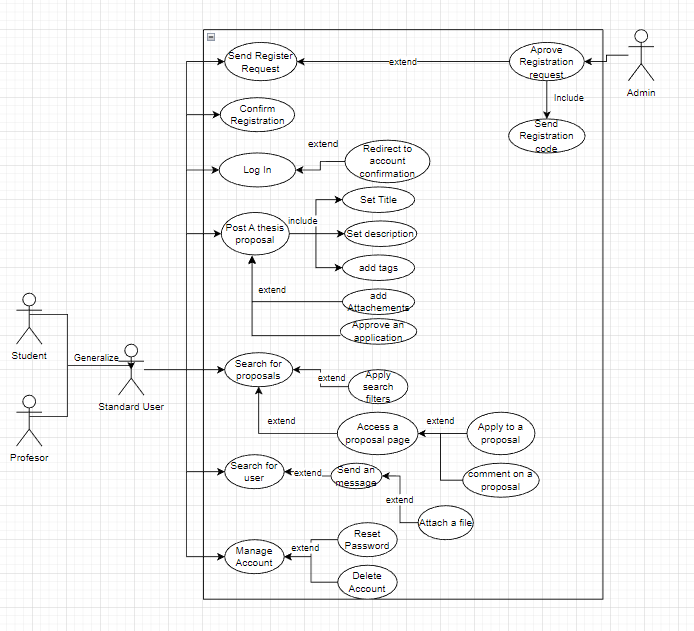
\includegraphics[scale=0.5]{images/StandardUserUseCase.png}
    \caption{Cazuri de utilizare pentru utilizatorii standard}
    \label{fig:stdUserDiagram}
\end{figure}
În diagrama de mai sus am ales să generalizez utilizatorul de tip Student și utilizatorul de tip Profesor ca un actor de tip „Utilizator standard” dat fiind faptul ca facilitățile disponibile celor  două tipuri de conturi sunt aceleași, diferențierea dintre cele două tipuri de conturi fiind totuși necesară din punct de vedere semantic(nu ar avea sens ca aplicația să permită unui student să coordoneze lucrări, sau unui profesor să aplice pentru tema propusă de alt profesor). Am încercat să cuprind în această diagramă toate cazurile de utilizare disponibile  unui utilizator standard cu scopul de a avea o imagine generala asupra facilitaților oferite de către platforma, voi analiza detaliat însă publicarea pe platforma a unei noi propunere de lucrări:



Acest caz de utilizare descrie procesul prin care noile propuneri de lucrări sunt adăugate pe platforma
\begin{itemize}
    \item{Actorii:
        \begin{enumerate}
            \item Utilizator standard
        \end{enumerate}}
    \item{Precondi\c tii:
        \begin{enumerate}
            \item Utilizatorul este de tip Profesor sau Student
            \item Contul acestuia trebuie să fi trecut atât de aprobarea înregistrării de către un administrator al platformei cât și confirmarea acesteia de către utilizator
            \item Utilizatorul este autentificat pe platformă
        \end{enumerate}}
    \item{Scenariu:
        \begin{enumerate}
            \item Accesarea paginii pentru crearea unei propuneri de licență
            \item Introducerea unui Titlu
            \item Introducerea unei Descrierii
            \item {Selectarea etichetelor potrivite temei propuse din lista de etichete disponibile
                \begin{enumerate}
                    \item utilizatorul este nevoit să selecteze cel puțin o etichetă pentru a continua
                \end{enumerate}}
            \item Opțional: Adăugarea eventualelor atașamente utile pentru descrierea temei propuse celorlalți utilizatorii interesați
            \item Dacă oricare dintre câmpurile menționate mai sus este invalid (gol sau prea scurt) atunci utilizatorul este avertizat
            \item Noua propunere de lucrare este creata pe platformă
        \end{enumerate}}
    \item{Postcondi\c tii:
        \begin{enumerate}
            \item Noua propunere este adăugată în baza de date a platformei și devine vizibilă celorlalți utilizatori ai platformei, ei putând interacționa cu această
        \end{enumerate}}
\end{itemize}
\section{Cazuri de utilizare pentru administratori}
\begin{figure}[H]
    \centering
    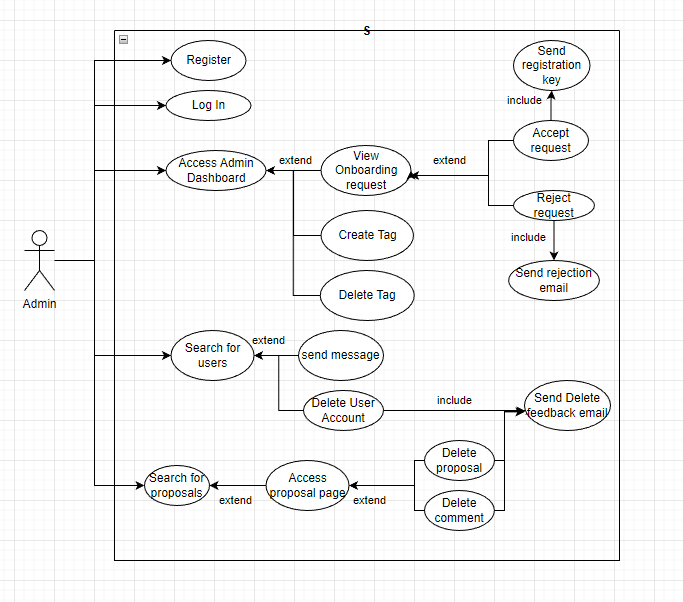
\includegraphics[scale=0.5]{images/AdminUserUseCase.png}
    \caption{Cazuri de utilizare pentru Administratori}
    \label{fig:adminUseCaseDiagram}
\end{figure}
Administratorii sunt utilizatorii cu privilegii ridicate, care au posibilitatea și responsabilitatea să gestioneze accesul celorlalți utilizatorii la platformă și să modereze conținutul acesteia pentru a păstra calitatea conținutului platformei la standardele universității și a unui mediu academic (eliminarea potențialelor postări/comentarii inadecvate scopului platformei), acest tip de conturi este gândit ca unul strict administrativ neavând astfel capacitatea de a:
\begin{itemize}
    \item Publica propuneri de lucrări.
    \item A aplica pentru propunerile existente sau de a lasă comentarii asupră acestora.
\end{itemize}
funcționalitățile comune cu conturile de utilizator standard fiind doar:
\begin{itemize}
    \item Autentificarea.
    \item Căutarea și accesarea  propunerilor de lucrări de pe platformă.
    \item Trimiterea de mesaje celorlalți utilizatori.
\end{itemize}
Am ales de asemenea că pentru diagramă de mai sus să abstractizez funcționalitatea ce ține de autentificare și trimiterea de mesaje, această fiind identică cu cea a conturilor standard reprezentate deja mai detaliat în diagrama precedentă, mai jos se poate revedea o analiză mai în detaliu a cazului de utilizare pentru aprobarea sau respingerea unei cererii de înregistrare.
\begin{itemize}
    \item {Actorii:
        \begin{enumerate}
            \item Administrator.
        \end{enumerate}}
    \item {Precond\c tii:
        \begin{enumerate}
            \item Utilizatorul are un cont de administrator pe platformă.
            \item Contul acestuia trebuie să fii trecut atât de aprobarea înregistrării de către un administrator al platformei cât și confirmarea acestuia de către utilizator.
            \item Utilizatorul este autentificat pe platformă.
            \item Există cel puțin o cerere de înregistrare pe platformă.
        \end{enumerate}}
    \item {Scenariul standard:
        \begin{enumerate}
            \item Utilizatorul accesează bordul de gestionare al administratorilor.
            \item Utilizatorul alege una dintre cererile de înregistrare.
            \item Utilizatorul verifica datele afișate in cererea de înregistrare.
            \item Utilizatorul verifica dovezile de identitate atașate de persoana care a inițiat cererea.
            \item Utilizatorul validează cererea.
            \item un email automat va fii trimis de către sistem utilizatorului care a inițiat cererea conținând un cod necesar pentru confirmarea înregistrării.    
        \end{enumerate}}
    \item {Postcondi\c tii:
        \begin{enumerate}
            \item Cererea o dată procesată va dispărea din bordul de gestionare al administratorilor.
            \item Un cod de confirmare a înregistrării este generat de către sistem și primit de către persoana care a inițiat cererea pe adresa de email folosită de către aceasta la crearea contului.
            \item Utilizatorul care a inițiat cererea are acum potențialul de își confirma contul, având apoi acces la restul funcționalităților de pe platformă.
        \end{enumerate}}
    \item {Scenariu alternativ:
        \begin{enumerate}
            \item Utilizatorul accesează bordul de gestionare al administratorilor.
            \item Utilizatorul alege una dintre cererile de înregistrare.
            \item Utilizatorul verifică datele afișate în cererea de înregistrare.
            \item Utilizatorul verifică dovezile de identitate atașate de persoana care a inițiat cererea.
            \item Utilizatorul respinge cererea.
            \item Utilizatorul este nevoit să justifice decizia de a respinge cererea.
            \item Un email de informare împreună cu justificarea respingerii oferită de către administratorul care a procesat cererea respectivă este trimis.
        \end{enumerate}}
    \item {Postcondi\c tii:
        \begin{enumerate}
            \item Cererea o dată procesată vă dispărea din bordul de gestionare al administratorilor.
            \item Contul nu a fost creat și un email de informare a fost trimis de către sistem.
        \end{enumerate}}
\end{itemize}
\section{Design-ul bazei de date}
\subsection{Privire de ansamblu}
\begin{figure}[H]
    \centering
    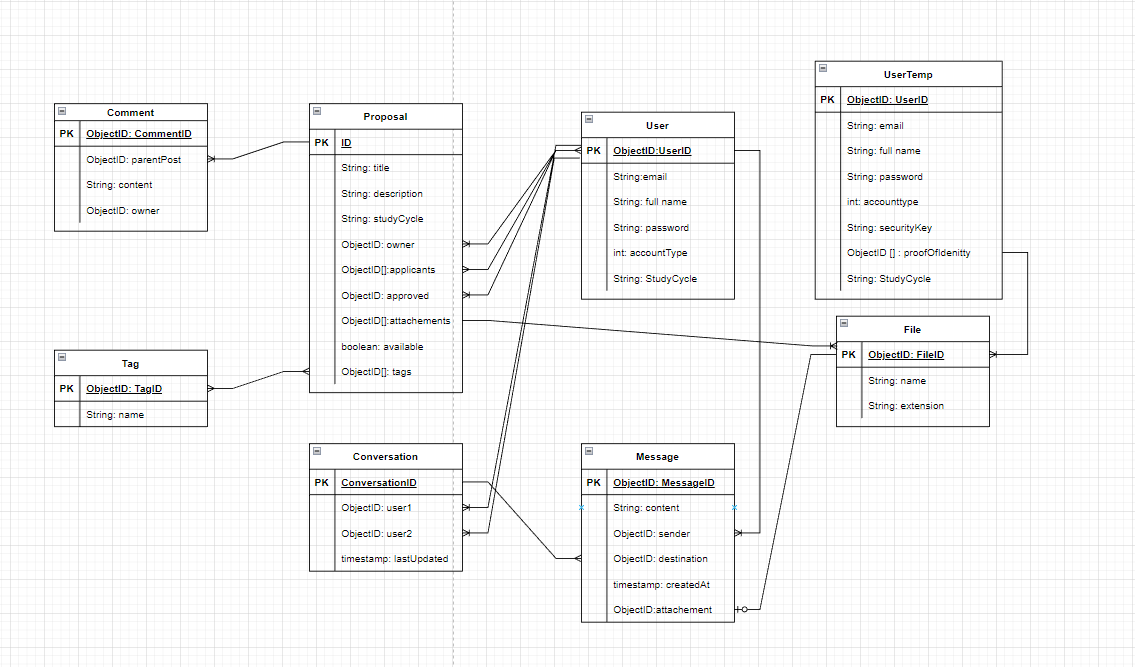
\includegraphics[scale=0.4]{images/DB_Diagram.png}
    \caption{Diagrama bazei de date}
    \label{fig:dbDiagram}
\end{figure}
Mai jos se poate regăsii o scurta descriere a fiecărei colecții regăsite în diagrama de mai sus
\subsection{Analiza colec\c tiilor din baza de date}
\subsubsection{User}
În această colecție vor fi stocate toate documentele care conțin informații despre utilizatorii aplicației, informații precum:
\begin{itemize}
    \item Nume.
    \item Email.
    \item Parola.
    \item Tip de utilizator (Profesor, Student sau Administrator).
    \item Ciclu de studiu(Licen\c ta sau Master)    
\end{itemize}
parolele sunt de asemenea trecute printr-un algoritm de „hashing”\footnote[1]{ in acest context un proces unidirectional si determinist de a mapa un \c sir de caractere la unul nou, de lungime fixa si cu un aspect complet aleatoriu pentru un eventual actor malitios care a ob\c tinut access la baza de date} înainte de a fii stocate din motive de securitate.
\subsubsection{UserTemp}
În această colecție sunt stocate cererile de înregistrare pe platformă, pe lângă câmpurile din colecția „User” avem un câmp în plus care va stoca o cheie de confirmare și referințe către dovezile de identitate aferente cererii din colecția de fișiere, în momentul când utilizatorul creează o cerere de înregistrare pe platformă un document nou va fii creat în această colecție având câmpul cheii de confirmare nul, o dată validată cererea de către administrator o cheie de confirmare va fii generată pentru acest utilizator și transmisă acestuia prin email, odată cu confirmarea înregistrării de către utilizator folosind cheia primită un document nou va fii creat în colecția "User" iar cel aferent cererii de înregistrare va fii șters din colecția „UserTemp”.
\subsubsection{Comment}
În această colecție sunt stocate comentariile de pe platformă, pe lângă conținutul comentariului se mai stochează și o refererin\c ta către utilizatorul care a postat comentariul și către propunerea de tema asupra căreia a fost lasat comentariul.
\subsubsection{Tag}
În aceasta colecție se găsesc etichetele pe care un utilizator le poate atașa unei propuneri la creare, ștergerea și adăugarea de documente noi în aceasta colecție este rezervată exclusiv administratorilor
\subsubsection{Conversation}
Această colecție servește funcționalita\c tii de mesagerie a platformei, aici sunt stocate conversațiile (doar membrii, nu și conținutul) de pe platformă, împreuna cu o data care reprezintă data și timpul ultimului mesaj nou în aceea conversație(necesar pentru afișarea conversațiilor unui utilizator în ordine cronologică.
\subsubsection{Message}
Această colecție stochează mesajele trimise de către utilizatorii, atributul „sender” conține id-ul utilizatorului care a trimis mesajul iar cel de „destination„ conține id-ul conversației în care a fost trimisă, utilizatorul   care doreste sa trimita un mesaj nou trebuie evident să fie un membru al acelei conversații.
\subsubsection{File}
Această colecție stochează numele fișierelor aferente platformei și extensia acestora, fișierele în sine fiind stocate în sistemul de fișiere al serverului, această colecție stocând doar referințe către acestea.
\subsubsection{Proposal}
această colecție stochează propunerile de teme de pe platformă, aceasta deține câmpuri primitive precum:
\begin{itemize}
    \item Descriere.
    \item Titlu.
    \item Ciclu de studiu.
    \item Disponibilitate.
\end{itemize}
dar și referințe către alte colecții precum:
\begin{itemize}
    \item "owner” reprezintă id-ul utilizatorului care a publicat propunerea de tema.
    \item „applicants” reprezintă un vector de id-uri ale unor utilizatori care au aplicat pentru propunerea în cauză.
    \item „attachaments” un vector de id-uri către fișierele aferente propunerii.
    \item „tags” conține referințe către etichetele atașate propunerii.
    \item „approved” conține o referința către utilizatorul a cărui aplicație a fost aprobată de către „owner” această referința este nula la creare și rămâne așa până când o aplicație este aprobată.
\end{itemize}
\chapter{Detalii de implementare}
\section{Tehnologiile alese}
\subsection{Frontend}
\subsubsection{Javascript}
Javascript este un limbaj de programare interpretat conceput inițial pentru a rula în browser cu scopul de a
manipula conținutul paginilor web si de a facilita astfel aplicații web cu conținut dinamic.

Acesta este un limbaj de programare de nivel înalt, oferind facilități precum : tipizare dinamica, gestionare automată
a memoriei si suport atat pentru programare funcționala, tratand funcțiile ca obiecte de ordin prim,
căt si pentru programarea orientată pe obiecte. În plus Javascript dispune de o bibliotecă standard vastă care să acopere
majoritatea nevoilor dezvoltatorilor cu privire la funcșionalităti "low level", atat expresivitatea limbajului
căt si timpul relativ scurt de invațare a acestuia au contribuit la creșterea popularității sale.

În momentul de fața Javascript se regăsește ca unul dintre cele mai folosite limbaje de programare,
acesta fiind intre timp extins in afara limitelor unui browser datorita tehnologiilor precum React Native si NodeJS;

\subsubsection{React}
React este un framework pentru dezvoltarea interfețelor web
care are la bază conceptul unui DOM virtual care să servească ca o interfața/intermediar a DOM-ului browser-ului,
Acest DOM virtual este reprezentat nativ în Javascript si stochat în memoria sistemului client, făcând astfel
manipularea acestui DOM virtual de catre Javascript mult mai puțin costisitoare.

Un alt concept fundamental pentru react sunt componentele, acestea stănd la baza oricărui proiect react.
Componentele au în definiția lor atât o reprezentare in DOM-ul virtual cât si stare, starea in acest context
poate fii interpretată ca și elementele non-statice dintr-o pagină web, care depind de utilizator si acțiunile sale.
odată ce starea unei componente a fost modificată este inițiat un proces de reconciliere intre  DOM-ul virtual si DOM-ul
browser-ului în urma căruia doar părțile care difera dintre cele două DOM-uri sunt rerandate in pagina web, celelalte părți 
rămânănd intacte. Datorită acestui fapt aplicațiile react tind să ofere o experiență de utilizare fluidă in schimbul
unui consum de memorie crescut.

Componentele de tip react pot conține în definiția lor atât componente primitive cât
și alte componente compuse iar componentele pot împartași în mod selectiv parți din starea lor cu componentele
din care sunt compuse, în acest fel, componentele care depind de stare comună între ele nu sunt nevoite să
gestioneze această stare in paralel, ci, în mod uzual starea comună împreună cu responsabilitatea gestionării ei 
este elevată la cel mai apropriat părinte comun al acestora iar starea este transmisă mai apoi in cascadă spre componentele care depind de ea. 

Atăt procesul simplu de gestionare a stării căt și
posibilitatea de îmbricare a componentelor duc spre două principii fundamentale în filosofia react,
mai exact compozabilitate si reutilizabilitate, aceaste 2 principii dovedindu-se extrem de utile in gestionarea complexități.
Rata de adopție a react-ului a fost una foarte abruptă datorită funcționalitaților inovative pentru timpul lor pe care le-a adus acesta
fiind în momentul de față de departe cel mai popular frontend framework.

\subsubsection{CSS}

CSS (Cascading Style Sheets) este un limbaj pentru descrierea stilului paginilor web. Deși HTML-ul permite stilizarea elementelor individuale folosind atributul de stil (Inline Styling) 
această abordare devine ineficientă în cazul unui proiect de complexitate ridicată. În mod uzual, HTML-ul este utilizat pentru a defini doar scheletul paginii web, 
în timp ce aspectul paginii este delegat CSS-ului. 

CSS oferă funcționalități precum moștenirea stilurilor, posibilitatea de a grupa elementele, aplicarea de stiluri pe grupuri de elemente și un sistem intuitiv de rezolvare a conflictelor. 

Apariția CSS a reprezentat un pas uriaș în evoluția dezvoltării web, revoluționând practic acest domeniu. Deși există alternative precum Sass, 
Less și Stylus, acestea sunt, în esență, doar extensii ale CSS-ului, iar codul scris în aceste limbaje este compilat în CSS înainte de a fi procesat de către browser. 
CSS nu are, astfel, vreun competitor real în această perspectivă

\subsection{Backend}
\subsubsection{NodeJS}
NodeJS este un mediu de rulare dezvoltat pentru a permite execuția programelor scrise în Javascript direct de către sistemul de operare, acesta a fost dezvoltat cu asincronicitate ca o prioritate,
in special pentru operațiile de Intrare/Iesire de date (I/O) ele fiind principala motivație pentru dezvoltarea acestei tehnologii.

Creatorul nodeJS era nemulțumit de abordarea clasică din aceea perioadă de a gestiona operațiile de Intrare/Ieșire pe serverele web, mai exact abordarea în care pentru fiecare cerere primită un nou fir de execuție era creat, 
această abordare este ineficientă deoarece acele fire de execuție sunt blocate până la finalizarea operației I/O,
consumănd totuși resurse intre timp(memoria rezervată firului de executie si timpul de procesare folosit pe schimbarea de context). 

NodeJS a fost proiectat în schimb să ruleze pe un singur fir de execuție
având la baza o buclă de evenimente, interpretorul de Javascript trece prin fiecare linie de cod și când acesta întampină cod asincron, precum citirea dintr-o bază de date, deleghează operațiile în cauza sistemului de operare.

Bucla de evenimente rulează continuu si verifică dacă operațiile delegate sistemului de operare și-au terminat execuția, în caz afirmativ aceasta apelează o functie definita sa ruleze odata cu finalul executiei codului asincron aferent
(Callback function), Arhitectura NodeJS-ului este principalul motiv datorita caruia  acesta este recunoscut si apreciat pentru scalabilitatea sa. 

Desi o tehnologie relativ recentă, aceasta a avut o creștere in popularitate
remarcabilă, fiind astăzi unul dintre cele mai populare tehnologii pentru backend, atât popularitatea deja existentă a Javascript-ului cât și ușurința de a îl învața, împreună cu 
conveniența de a folosi un singur limbaj de programare atăt pe backend cât si pe frontend sunt principalele cauze ale popularității sale, coborând de astfel considerabil
bariera de intrare pentru dezvoltarea web, fiind un favorit pentru începatorii din acest domeniu.
\subsubsection{Express}
Express este un framework minimalist si neopinionat al nodeJS-ului dedicat pentru dezvoltarea serverelor web, acesta poate fii considerat minimalist deoarece oferă
o suită relativ mică de faciliăti, focusăndu-se pe anumite funcționalități generale, de exemplu: rutarea cererilor http, ușurând procesul de a lucra cu rute dinamice si oferind posibilitatea de a grupa rutele, un sistem
de gestiune a fluxului cerere-răspuns, și suport pentru șablonarea paginilor în cazul aplicațiilor unde randarea se face pe server.

Express prioritizează integrablitiatea și extensibilitatea să cu alte librării, delegănd comunității datoria de a dezvolta librării pentru a acoperii cazuri de utilizare specifice și dezvoltatorului datoria de a se documenta si alege "uneltele" necesare pentru proiectul său.

Acesta mai este descris si ca neopinionat deoarece își propune să nu împună dezvoltatorilor o anumită paradigmă, arhitectura software
sau set de convenții / "bune practici" lăsănd dezvoltatorilor atât liberatea cât și responsabilitatea de a alege acestea în funcție de particularitățile proiectului și a echipei în care lucrează. 

Abordarea liberală a expressului a rezultat intr-un ecosistem vast si in continua crestere in jurul sau, fiind astazi unul dintre cele mai populare librarii NodeJS folosite.

O functionalitate care sta la baza express-ului este support-ul pentru middleware, pentru fiecare ruta definita avem cel putin o functie care va fii apelata odata cu intrarea
unui cererii pe aceea ruta,
important este insa faptul ca express ne permite sa adaugam si o lista de functii intermediare care vor fii apelate secvential, oricare dintre acestea putand oprii prematur executia(de regula in cazuri de eroare) 
sau de a apela urmatoarea functie din lant, optional acestea pot si adauga/modifica date din cererea primita inainte de a apela urmatoare functie, 
acesta reprezentand un mecanism de a persista stare intre diferitele functii inmplicate in ciclul de viata al unei cererii, acest fapt crescand semnificativ potentiala modularitatea a codului
\subsubsection{MongoDB}
MongoDB este un sistem de gesitionare a bazelor de date de tip NoSQL bazat pe documente
(echivalentul rândurilor într-o baza de date de tip SQL) și colecții (echivalentul tabelelor în baze de date SQL), 
documentele sunt scrise în format BSON(Binary Javascript Object Notation), 
Acest format suportând obiecte(imbricarea obiectelor fiind suportată de asemenea) și vectorii 
de valorii primitive sau de obiecte in plus fata de tipurile primitive comune cu SQL, 
Acest fapt oferă o flexibilitate semnificativ mai mare în proiectarea 
unei baze de date spre deosebire de un DMBS de tip SQL, 
această flexibilitate vine însă la costul consistenței, o colecție nu impune 
în mod nativ o schemă asupră documentelor pe care le are în apartenentă, 
astfel în mod teoretic se poate ca două documente din aceiași colecție sa aiba o structura diferita, 
de regulă sunt impuse însă soluții de validare a operațiunilor de creare/modificare 
pentru a putea asigura o consecvența a datelor.
\subsubsection{Mongoose}
Mongoose este o librarie de mapare a datelor in obiecte (Object-Data Modeling), ODM-urile 
ofera o interfata de tip OOP in limbajul de programare ales pentru a interactiona cu baza de date NoSQL aleasa,
conditiia fiind evident ca ODM-ul ales sa suporte atat
limbajul de programare ales cat si baza de date. Mongoose ofera o interfata in javascript pentru 
a interactiona cu baze de date de tip MongoDB, pe langa aceasta convenienta de a putea comunica cu baza de date 
scriind cod direct in javascript si suita de functii care abstractizeaza detalii de implementare ale unor
nevoi comune(de exemplu findByIdAndDelete), acesta mai are un beneficiu foarte important  
deoarece ajuta in diminuarea principalului dezavatanj al MongoDB-ului, mai exact lipsa de consistenta.
Mongoose interactioneaza doar cu colectiile din baza de date pentru care are un model definit, la baza acestui 
model sta o schema definita in JSON pe care obiectele din aceea colectie ar trebui sa o respecte. Orice incercare
de a creea / modifica obiecte in asa fel incat nu vor respecta schema definita va genera o eroare, acest lucru 
nu rezolva in totalitate problema din pacate insa deoarece valideaza doar operatiile de scriere pe care acesta le primeste,  
baza de date putand fii inca modificata direct si astfel aceastqa ar putea ajunge intr-o stare inconsistenta. 
Practic mongoose garanteaza consistenta bazei de date doar daca scrierea in aceasta se fac in mod exclusiv
prin mongoose.
\subsection{General}
\subsubsection{HTTP}
HTTP(Hypertext Transfer Protocol) este un protocol de comunicare construit pe baza  protocolului TCP/IP cu scopul de a standardiza
comunicarea intre clienti si serverele web, acesta urmeaza modelul "cerere-raspuns", in care
clientul si server-ul stabliesc o conexiune, clientul apoi trimite o cerere serverului iar serverul trimite inapoi un raspuns,
dupa care conexiunea este inchisa, protocolul HTTP sta la baza web-ului acesta fiind protocolul folosit pentru marea majoritate
a traficului web, acesta are o limitare insa, cum conectiunea poate fii initiata doar de catre client, iar aceasta este inchisa automat odata cu
primirea raspunsului din partea serverului cererile de tip HTTP nu sunt potrivite pentru cazurile de utilizare unde se doreste ca serverul sa 
trimita mesaje catre client, cum ar fii in cazul de fata functionalitatea pentru mesagerie, in care se doreste ca serverul 
sa trimita clientului mesajele primite in timp real. Exista cateva "solutii" pentru a suporta aceasta functionalitae, cum ar fii HTTP polling
unde clientul trimite cereri catre server pentru a obtine mesajele noi la un interval fix de timp, problema cu aceasta abordare fiind
echilibrul dintre responsivitate si performanta, in aceasta abordare daca timpul de asteptare dintre cererii este prea lung atunci experienta utilizatorului
se degradeaza considerabil, insa daca cereriile sunt prea frecvente atunci performanta sistemului va avea de suferit, crescand drastic numarul de cererii
trimise in timp ce majoritatea acestora vor fii redundante.

O alta solutie ar fii HTTP long polling, unde se trimite o singura cerere, iar serverul blocheaza acel fir de executie(fiind creat un fir de executie diferit pentru fiecare cerere) pana cand
acesta are date de trimis clientului, dupa care raspunsul este trimis si conexiunea este inchisa, iar apoi clientul initiaza o noua astfel de cerere,
aceasta abordare este mai eficienta decat prima insa este tot suboptima, deoarece o buna parte din resursele serverului vor fii blocate la orice moment dat.
\subsubsection{WebSockets}
WebSockets este un protocol construit cu scopul de a rezolva problemele cauzate de limitarile protocolului HTTP, construit tot pe baza TCP/IP acesta ofera 
posibilitatea unei comunicari bidirectionale si cu latenta redusa intre client si server, facand astfel aplicatiile web care necesita comunicare in timp real
fezabile, in acest protocol conexiunea dintre client si server este proiectata sa persiste iar atat clientul cat si serverul pot sa trimita evenimente
celuilalt oricand iar aceste mesaje sunt mult mai rapide deoarece acestea nu trebuie sa includa "bagajul" necesar pentru stabilirea unei conexiuni noi 
spre deosebire de http
\section{Manual de Implementare}
\subsection{Backend}
\subsubsection{Arhitectura sistemului}
fisierele care contin codul sursa sunt impartite logic in urmatoarele categorii:
    \begin{itemize}
        \item {
            Models: acest folder contine modelele mongoose aferente colectiilor din baza de date
        }
        \item {
            Controller: in acest folder se regasesc functiile definite pentru a trata cererile primite
        }
        \item{
            Routes: aici sunt definite rutele pe care le accepta serverul si sunt legate de functiile care ar trebui sa ruleze la apelarea rutelor respective
        }
    \end{itemize}
    dupa cum se poate observa in figura 4.1 exista o mapare de aproape 1:1 intre modele si controllere,
    arhitectura implementata a fost in mare parte inspirata de catre MVC(Model View Controller), functiile care creaza/returneaza/modifica sau sterg
    obiecte ce apartin de un anumit model sunt grupate sub un singur fisier numit controller legat logic de model-ul aferent, aceasta implementare
    nu respecta in totalitate arhitectura MVC totusi, deoarece backend-ul in acest caz este un rest api care comunica in mod exclusiv prin JSON
    fisierele statice(HTML, CSS si javascript) nefiind sub responsabilitatea acestuia, partea de View lipsind astfel complet din aceasta arhitectura.
    livrarea fisierelor statice ce tin de frontend sunt delegate in momentul de fata serverului http local care vine la pachet cu mediul de dezvoltare react,
    acesta este conceput insa doar ca o solutie pentru testarea si dezvoltarea locala, pentru a livra in productie aceste fisiere ce tin de frontend
    mai intai codul react trebuie compilat intr-un build optimizat (cu ajutorul aceluiasi mediu de dezvoltare) iar apoi livrat de catre un server http dedicat.
    O solutie posibila ar fii configurarea serverului de express pentru a livra si aceste fisiere statice, insa aceasta solutie nu este favorabila deoarece
    reduce scalabilitatea intregului sistem si ar reprezenta deasemenea un "single point of failure", o solutie mai buna ar fii folosirea unui server http dedicat pentru servirea de continut static
    precum NGINX si configurarea acestuia ca si un reverse proxy pentru serverul de express, permitand astfel adaugarea mai multor instante ale serverului de back end
     la nevoie, serverul reverse proxy avand atat scopul de a livra continutul static dar funtionand si ca un load balancer
    \begin{itemize}
        \item Config: aici se regasesc functii pentru conectarea la baza de date 
        si conectarea serverului de express cu serverul de SMTP pentru functionalitatiile ce implica trimiterea de email-uri
        \item Middleware: acest folder contine functiile intermediare rulate inainte de cele din controller, in mare parte functionalitate pentru validarea request-ului
        dar sunt si unele functii menite pentru a aduaga informatii in request-ul primit de la client
        \item Utils: aici se regaseste de regula cod necesar/util care nu potriveste insa nici unei alte locatii din punct de vedere semantic.
        In cazul de fata o clasa care extinde clasa de baza "Error", care primeste ca si attribut pe langa un mesaj de eroare si un code de status
        util in generarea si tratarea erorilor intampinate de un server web
    \end{itemize}
    \begin{figure}[H]
        \centering
        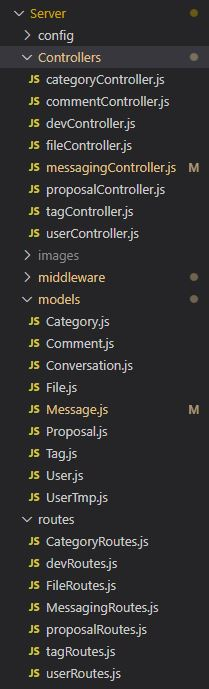
\includegraphics[scale=1]{images/MVC.JPG}
        \caption{Structura codului backend}
        \label{fig:backEndCodeStructure}
    \end{figure}
    \subsubsection{fluxul de control}
    Pentru a putea intelege mai bine modul de functionarea a serverului, consider ca ar fii utila urmariea cap-coada a ciclului de viata a unui request, 
    in cazul de fata o cerere care consta in aprobarea unei aplicatii ar fii ceea mai potrivivita.
    
    Odata cu pornirea serverului, acesta creaza o instanta noua de express, si ii specifica acesteia ca pentru oricare cerere a carei 
    destinatii incepe cu "api/proposal" sa foloseasca rutele definite in proposalRoutes.
    \begin{lstlisting}[language=Javascript]
        import express from "express";
        import proposalRoutes from "./routes/proposalRoutes.js";

        const app = express();
        app.use("/api/proposal", proposalRoutes);
    \end{lstlisting}
    In acest set de rute o avem pe urmatoarea definita: "/:proposalID/approve" unde ":proposalID" este un parametru, acesta nu are o valoare predefinita,
    ci este mai degraba un substituent, practic orice request de tipul: /api/proposal/<id>/approve  
    unde id poate sa ia orice valoare va intra pe aceasta ruta, valoarea acestuia fiind facuta disponibila functiilor care
    trateaza cererea, acestea putand accesa proprietatea req.params.proposalID
    \begin{lstlisting}[language=Javascript]
        import express from "express";
        import { auth } from "../middleware/auth.js";
        import {addProposalToReq,
            isProposalOwner,
            validateApproval} from "../middleware/validators/proposalValidator.js";
        import {approveApplication} from "../Controllers/proposalController.js";
        import { isAuthorized } from "../middleware/validators/userValidator.js";

        const router = express.Router();
        router.put("/:proposalID/approve", auth,
            addProposalToReq,
            isProposalOwner,
            isAuthorized,
            validateApproval,
            approveApplication);
        export default router;
    \end{lstlisting}
    odata intrat un astfel de request, prima functie care se apeleaza este ce de autorizare,
    pentru a vorbi despre aceasta insa, consider ca o scurta explicatie despre Json Web tokens (JWT)
    este necesara deoarece aceasta tehnologie sta la baza sistemului de autentificare si autorizare.
    
    In urma unei autentificari reusite
    serverul genereaza un hash pe baza incarcaturii token-ului (payload-ul, in cazul de fata id, tip cont si ciclu de studii)
    timpul si o cheie secreta data serverului ca si variabila de mediu (environment variable), token-ul nu poate fii descifrat
    fara a avea access la cheia secreta folosita pentru a genera hash-ul iar token-ul nu poate fii alterat de catre
    un eventual actor malitios deoarece oricare alterare va rezulta intr-un hash invalid
    (modificarea unui singur caracter oarecare din cele folosite pentru generarea token-ului va genera un hash complet diferit, astfel
    nu se poate "ghici" ce modificare pot fii aduse unui token deja existent pentru a ii modifica payload-ul), odata acest token primit
    clientul il salveaza in memoria locala si il ataseaza la fiecare request, serverul cunoscand secretul cu care a fost "semnat" token-ul
    il poate descifra pentru a avea access la acest payload si astfel identifica cine este utilizatorul care a initiat request-ul in cauza.
    Revenind la functia noastra, aceasta verifica daca requet-ul primit contine un header de autorizare de tip "Bearer token",
    si daca da incearca sa il descifreze folosind codul secret, in cazul in care header-ul este prezent si poate fii descrifrat(este valid) atunci
    adauga in request payload-ul token-ului si apeleaza urmatoarea functie din lant, in caz contrar trimite clientului un raspuns de tip eroare si opreste procesare acelui request
    \begin{lstlisting}[language=Javascript]
        import jwt from "jsonwebtoken"

        function auth (req, res, next){
            if(req.headers.authorization &&
            req.headers.authorization.startsWith("Bearer")){
                try {
                    let token = req.
                     headers.
                     authorization
                     .split(" ")[1];
                    req.user = jwt
                     .verify(token, process.env.AUTH_SECRET);
                    next();
                } catch (error) {
                    console.log(error)
                    return res.status(500).json(error);
                }
            }
            else{
                return res.
                 status(400)
                 .json({msg:"auth token not found or invalid"})
            }
        }
    \end{lstlisting}
    urmatorul pas este sa verificam daca id-ul primit ca si parametru este unul valid, mai intai verificam daca s-a primit o valoare pentru acest ID sau acesta este null
    iar in caz afirmativ, obtinem din baza de date obiectul aferent acelui ID si il atasam cererii in acelasi mod ca si in pasul anterior 
    iar intr-un final apelam urmatoarea functie din lant. In cazul insa in care nu a fost oferit un ID sau nu exista acest ID in baza de date, returnam din nou eroare
    \begin{lstlisting}[language=Javascript]
    async function addProposalToReq(req, res, next){
        try {
            validateString(req.params.proposalID);
            const proposal = await Proposal
                .findById(req.params.proposalID)
                .populate({
                    path: "owner",
                    model: "User"
            })
            if(!proposal){
                throw new customError(```the proposal ID provided
                 does not exist```, 400);
            }
            req.post = proposal;
            next();
        } catch (error) {
            if(error instanceof customError){
                return res
                 .status(error.statusCode)
                 .json({msg: error.message})
            }
            console.log(error);
            return res.status(500).json(error);   
        }
}
    \end{lstlisting}
    urmatorul pas este sa verificam daca utilizatorul care a initiat cererea este si detinatorul propunerii de teme,
    in caz afirmativ, se adauga un nou atribut in request, numit auth si este setat ca adevarat.
    La final se apeleaza urmatoarea functie din lant indiferent de rezultatul conditiei
    \begin{lstlisting}[language=Javascript]
        async function isProposalOwner (req, res, next){
        try {
            if(req.user.id == req.post.owner._id){
                req.auth = true;
            }
            next();
        } catch (error) {
            return res.status(500).json({msg: error});
        }
    \end{lstlisting}
    apoi se verifica daca utilizatorul este autorizat sau nu pentru a initia cererea in cauza, acest lucru se face verificand
    daca vre-o functie anterioara lui "isAuthorized" a setat deja attributul "req.auth" ca adevarat, in caz afirmativ
    acesta apeleaza doar functia urmatoare din lant, iar in caz contrar returneaza o eroare de tipul "permisiuni insuficiente"
    aceasta abordare simplifica seminificativ implementarea unu sistem de permisiuni complex, dat fiind modularitatea sa
    acesta presupune doar definirea unor middleware-uri care verifica unele conditii simple, si apoi la definirea rutei
    acestea se pot inlantuii in functie de nevoie, un exemplu pentru asta ar putea fii: o ruta pentru stergerea unui comentariu
    si o ruta pentru editarea unui comentariu, ar avea sens ca atat persoana care a postat comentariul, 
    cat si persoana care detine postarea in care a fost postat comentariul, cat si un administrator sa poata sterge comentariul in cauza 
    insa doar persoana care a postat comentariul ar trebui sa aibe permisiunea de a ii modifica continutul, in acest context
    ambele cazuri se pot rezolva implementand urmatoarele functii: isCommentOwner, isProposalOwner, isAdmin in acelasi mod ca si in pasul precedent
    iar apoi pentru ruta de stergere apelam urmatoarea lista de functii "..., isCommentOwner, isProposalOwner, isAdmin, isAuthorized, ..."
    iar pentru cea de editare apelam doar "...,isCommentOwner, isAuthorized, ..."
    \begin{lstlisting}[language=Javascript]
        async function isAuthorized(req, res, next){
        try {
            if(!req.auth)
                return res
                 .status(400)
                 .json({msg: ```Insufficient permissions
                 to proceed with this request```});
            next();
        } catch (error) {
            console.log(error);
            return res.status(500).json({msg: error});
            
        }
    }
    \end{lstlisting}
    dupa autorizare, urmatorul pas este validarea cererii, functia verifica daca propunerea respectiva are deja o aplcatie aprobata
    si daca id-ul utilizatorului aplicant lipseste din baza de date, daca cel putin una dintre aceste doua sunt adevarate atunci functia va returna o eroare si va oprii executia
    in caz contrar, se apeleaza ultima functie din acest lant
    \begin{lstlisting}[language=Javascript]
        async function validateApproval(req, res, next){
        try {
            if(req.post.approved){
                throw new customError(```you have already approved
                 an application for this particular proposal```, 400);
            }
            const user = await User
            .findById(req.body.applicantID);
            if(!user){
                throw new customError(```the provided applicant ID
                 does not exist```, 400);
            }
            next();
        } catch (error) {
            if(error instanceof customError){
                return res
                .status(error.statusCode)
                .json({msg: error.message})
            }
            console.log(error);
            return res.status(500).json(error);   
        }
    }
    \end{lstlisting}
    pasul final, atributul "approved" al postari este modificat din null in id-ul utilizatorului a carui aplicatie a fost aprobata
    si apoi functia trimite un raspuns cu un mesaj de success clientului
    \begin{lstlisting}[language=Javascript]
        async function approveApplication (req, res){
        try {
            const post = req.post;
            post.approved = req.body.applicantID;
            await post.save()
            return res
             .status(200)
             .json({msg: "application approved!"});
        } catch (error) {
            console.log(error);
            return res.status(500).json(error);
        }
}
    \end{lstlisting}
\subsection{frontend}
\subsubsection{arhitectura sistemului}
Codul sursa este impartit in urmatoarele categorii:
\begin{itemize}
    \item Pages: aici se regasesc componentele React aferente paginilor platformei,
    acestea sunt componentele la cel mai inalt nivel de abstractizare, fiind compuse la randul lor
    din alte componente React de nivel inalt.
    \item css: In acest folder se regasesc toate fisierele ce tin de stilizarea componentelor, codul sursa de css
    a fost impartit in fisiere in functie de pagina de care apartine
    \item api: Acest folder contine functiile folosite pentru trimiterea de cererii http catre backend, functiile respective sunt importate in anumite componente React 
    si apelate in urma unor evenimente(de exemplu la incarcarea initiala a componentei sau in urma unei apasari de buton de catre utilizator). 
    Comunicarea cu server-ul pentru functionalitatea de mesagerie nu se regaseste aici insa, pentru aceasta componenta comunicarea cu serverul este realizata folosind protocolul 
    WebSockets ci nu http, evenimentele dupa care client-ul "asculta" pot fii definite doar dupa stabilirea unei conectiuni cu clientul, din acest motiv
    logica ce tine de mesagerie a fost incapsulata in pagina dedicata pentru mesagerie.
    \item Images: Aici se regasesc  imaginile ce tin de aplicatia web in sine, acest folder este diferit de cel ce contine 
    atasamentele aferente  mesajelor/propunerilor de pe platforma. In cazul de fata acest folder contine logo-ul aplicatiei
    \item Utils: In acest folder se regasete functionalitatea de validare de pe front, aceste functii sunt apelate inainte de trimiterea unor cererii catre server. 
    Este de preferat identificarea cererilor gresite preventiv pe cat de mult posibil, deoarce daca suntem intr-o situatie in putem stii sigur ca cererea va rezulta intr-o eroare inca de pe front-end(un camp obligatoriu lipseste de exemplu), 
    atunci clientul poate sa il anunte pe utilizator direct, evitand astfel trimiterea unei cererii si asteptarea unui raspuns pentru ea.
    reducand in acest fel atat timpul de asteptare al utilizatorului cat si incarcatura pe care o suporta server-ul
    \item Components: In acest fisier sunt grupate restul componentelor de tip React.
    Aici se regasesc atat componente simple (a caror definitii detin doar elemente primitive) cat si componente de nivel inalt 
    (a caror definitie contin alte componente de tip React). 
    Pentru a exemplifica diferenta dintre cele doua tipuri putem compara doua astfel de componente, cum ar fii Checkbox si taglist:
    dupa cum se poate observa mai jos componenta Checkbox este compusa dintr-un div(container) si un element de tip p (paragraf)
    ambele putand fii considerate elemente primitive.
    \begin{lstlisting}[language=Javascript]
    export const Checkbox = ({text,
     tagID,
     checked,
     onClick}) => {
        function handleChange(){
            onClick({tagID, text});
        }

        return(
            <div className = {checked ?
            "checkbox-checked"
            :"checkbox-unchecked"}
            onClick={handleChange}>
                <p>{text}</p>
            </div>
        )
    }
    \end{lstlisting}
    Componenta TagList insa are in definitia sa alte componente compuse de tip React dupa cum se poate vedea, 
    din acest motiv poate fii considerata ca o componenta de nivel inalt
    \begin{lstlisting}[language=Javascript]
    export const TagList = ({tags,
     onChange,
     resetView,
     resetTags,
     categoryID})=>{
        return (
            <div className="taglist">
                <button onClick={resetView}
                className="checkbox-unchecked">
                    back to categories
                </button>
                <button onClick={resetTags}
                className="checkbox-unchecked">
                    reset tags
                </button>
                <Divider orientation='horizontal' />
                <div className="taglist-tags">
                {
                    tags.map(tag =>{
                        return (tag.category == categoryID) ?
                        <Checkbox text={tag.text}
                            tagID = {tag.id}
                            checked = {tag.checked}
                            onClick = {onChange}
                            key = {tag.id} >
                        </Checkbox> : null;
                    }) 
                }
                </div>
            </div>
        )
}
    \end{lstlisting}
\end{itemize}
\subsubsection{Ierarhia componentelor}
prima componenta din ierarhie este App, aceasta incorporeaza defapt intreaga aplicatie, react-ul genereaza "aplicatii cu o singura pagina" (Single Page Applications),
mai exact la accesarea pagini se trimite catre client codul necesar pentru a putea genera intreaga aplicatie, in mod clasic clientul
face o cerere spre server si primeste codul html, css si javascript pentru fiecare navigare intre pagini, fiecare pagina fiind separata, React insa
doar manipuleaza dom-ul browser-ului pentru a randa subcomponente diferite a acestui element de radacina in functie de URL pe care se afla utilizatorul si simuland 
astfel comportamentul unei aplicatii cu mai multe pagini
\begin{lstlisting}[language=Javascript]
    import { AuthPage } from './Pages/AuthPage';
    import { HomePage } from './Pages/HomePage';
    import { CreateProposalPage } from './Pages/CreateProposalPage';
    import { ProposalPage } from './Pages/ProposalPage';
    import { MessagesPage } from './Pages/MessagesPage';
    import { AdminDashboard } from './Pages/AdminDashboard'

    function App() {
    return (
        <Router>
            <Routes>
            <Route path='/' element={<HomePage/>}/>
            <Route path='/auth' element={<AuthPage/>}/>
            <Route path='/proposal/create' element = {<CreateProposalPage/>}/>
            <Route path='/proposal/:proposalID' element ={<ProposalPage/>}/>
            <Route path="/messages/" element = {<MessagesPage/>}/>
            <Route path="/admin/" element = {<AdminDashboard/>}/>
            </Routes>
        </Router>
    )
}
export default App;   
\end{lstlisting}
in cazul de fata pentru fiecare ruta definita este asociata o componenta de tip pagina.
Una dintre ele este pagina propunerilor, aceasta este o ruta dinamica, id-ul propunerii fiind dat ca parametru.
Aceasta pagina are in componenta sa:
\begin{itemize}
    \item Bara de navigare: aceasta componenta contine butoane pentru redirectarea spre celalalte pagini si este regasita dealtfel in toate celelalte pagini
    \item ProposalItem: aceasta componenta contine datele propunerii, mai exact: titlu, descriere, detinator, ciclu de studii, etichete(tags) si atasamentele propunerii
    \item CommentSection: aceasta componenta contine atat lista de comentarii de pe platforma cat si componenta pentru adaugarea comentariilor noi
\end{itemize}
\begin{lstlisting}[language=Javascript]
    <div className="ProposalPage">
        <Navbar/>
        <VStack>
            <div className="proposal-page-main-main">
                {!loading && <ProposalItem 
                    proposalData={proposal} 
                    updateProposalApplications = {updateProposalApplications} 
                    updateProposalApproved = {updateProposalApproved}/>}
                <CommentSection proposalID={proposalID}/>
            </div>
        </VStack>
    </div> 
\end{lstlisting}
componenta "Comment-section" primeste de la parinte id-ul cererii, si la initierea acesteia
trimite o cerere spre server pentru a obtine lista de comentarii aferente propunerii, itereaza 
apoi prin lista primita si genereaza un CommentItem(comentariu) pentru fiecare element din lista.
\begin{lstlisting}[language=Javascript]
    {
    !isloading &&
    <div className="Comment-section">
        <div className="Comments" ref={commentListRef}>
            {
                commentList.map(comment =>{
                    return <CommentItem 
                     key={comment._id} 
                     comment={comment}/>
                })
            }
        </div>
        <div className="Add-comment">
            <textarea id="message" 
             name="message" 
             placeholder= {"press <Shift> + <Enter> to send the message ..."}
             ref={textboxRef} 
             onKeyDown={(e)=>{handleChange(e)}}>
            </textarea>
        </div>
    </div>
    }
\end{lstlisting}
Iar componenta "comment-item" primeste de la componenta parinte continutul comentariului ca si stare
si pe baza acestuia se genereaza continutul comentariului, sintaxa JSX permite definirea de blocuri de cod javascript(intre acoloade)
aceste blocuri permit sa generam continut dinamic, componentele putand astfel avea variabile in definitiile lor.
Aceasta sintaxa ne permite si sa randam in mod conditional un element, dupa cum se poate vedea mai jos, 
iconita aferenta autorului comentariului este definita conditional folosind operatorul tertiar in functie de tipul de cont 
al autorului.
\begin{lstlisting}[language=Javascript]
import { GiTeacher } from "react-icons/gi";
import { FaUserGraduate } from "react-icons/fa";
export const CommentItem = ({comment}) =>{
    return(
        <div className="comment-item">
            <p>{comment.content}</p>
            <div className="comment-item-footer">
                <div className=
                 "comment-item-footer-nameAndType">
                    {comment.owner.type === "Student" ?
                     <FaUserGraduate/>:
                     <GiTeacher/>}
                    <p>{comment.owner.name}</p>
                </div>
                <p>{new Date(comment.postedAt)
                 .toLocaleDateString("ro-RO", 
                 { 
                    day: "numeric",
                    month: "numeric",
                    year: "numeric"
                 })
                }</p>
            </div>
        </div>
    )
}
\end{lstlisting}
\section{manual de utilizare}
Primul pas necesar pentru a putea folosi platforma este trimiterea unei cereri de inregistrare, pentru asta este necesar
ca utilizatorul sa acceseze formularul de inregistrare si sa completeze urmatoarele informatii:
\begin{itemize}
    \item Nume si prenume
    \item adresa de email
    \item parola
    \item tipul de cont (putand alege intre Student Profesor si Administrator)
    \item in cazul in care tipul de cont este student, atunci mai trebuie ales si ciclul de studii
    \item atasamente continand dovezi de identitate
\end{itemize}
\begin{figure}[H]
    \centering
    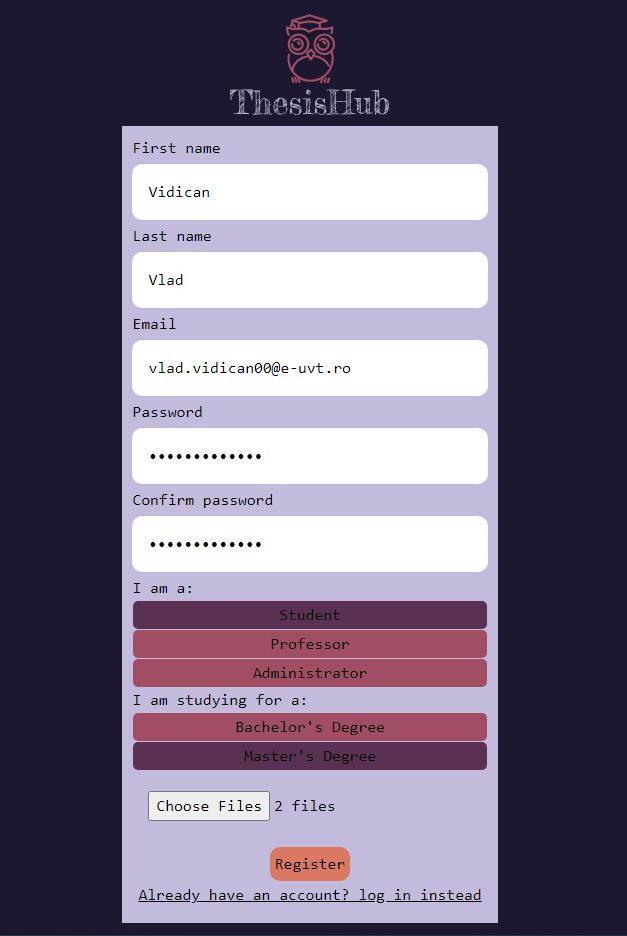
\includegraphics[scale=0.5]{images/RegisterForm.png}
    \caption{formular de inregistrare}
\end{figure}

Apoi utilizatorul va primi un cod de securitate pe adresa de email folosita la crearea contului, pe care va trebui sa il introduca
in interfata deschisa dupa trimiterea cererii, aceasta interfata ii permite de asemenea utilizatorului sa solicite un cod nou de securitate
in cazul in care mail-ul initial nu a fost livrat.
\begin{figure}[H]
    \centering
    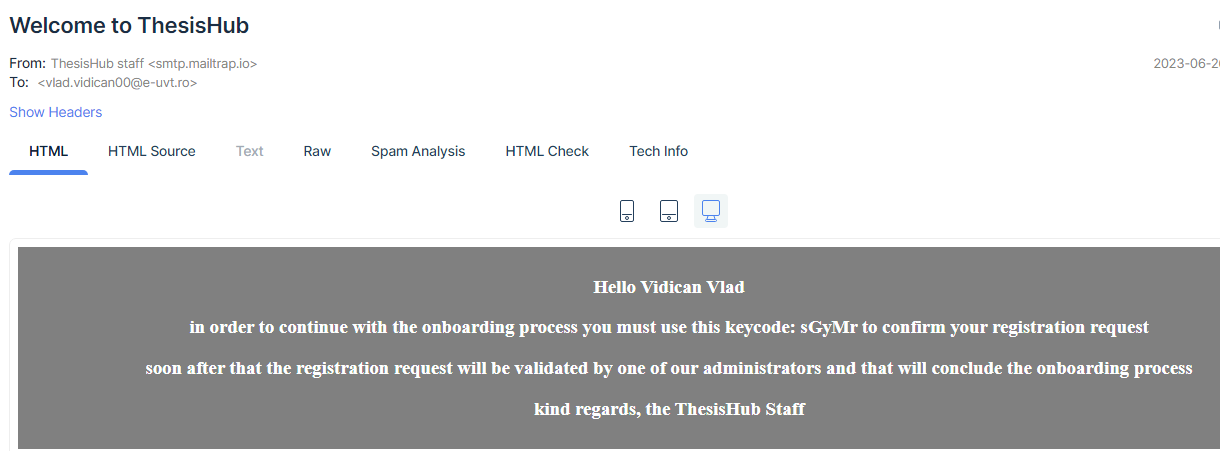
\includegraphics[scale=0.5]{images/RegisterEmail.png}
    \caption{exemplu email primit la inregistrare}
\end{figure}
\begin{figure}[H]
    \centering
    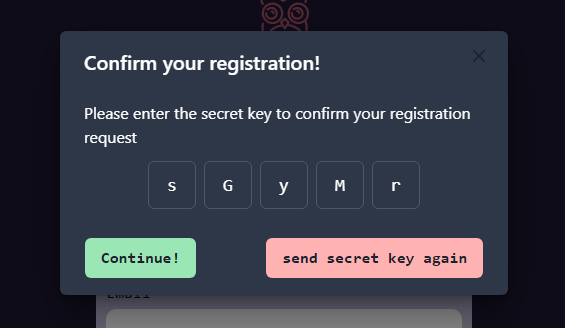
\includegraphics[scale=0.5]{images/SecurityKey.png}
    \caption{interfata pentru introducerea codului de securitate}
\end{figure}

dupa ce utilizatorul introduce codul secret cererea lui de inregistrare este confirmata, 
ceea ce inseamna ca aceasta va fii acum vizibila in bordul de gestionare a administratorilor (admin dashboard)
si urmeaza sa fie revizuita de catre unul din administratorii platformei, pentru acest pas utilizatorul nu are nimic de facut,
odata ce cererea ii va fii aprobata acesta  se va putea autentifica pe platforma, acestia 
vor primi de asemenea un email de informare in legatura cu acest eveniment.
\begin{figure}[H]
    \centering
    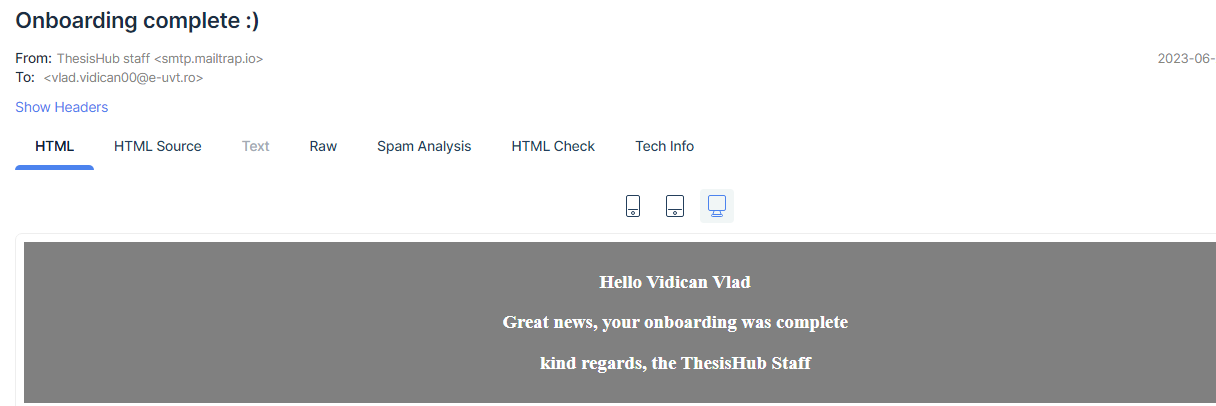
\includegraphics[scale=0.5]{images/OnboardingComplete.PNG}
    \caption{exemplu email de informare}
\end{figure}
\begin{figure}[H]
    \centering
    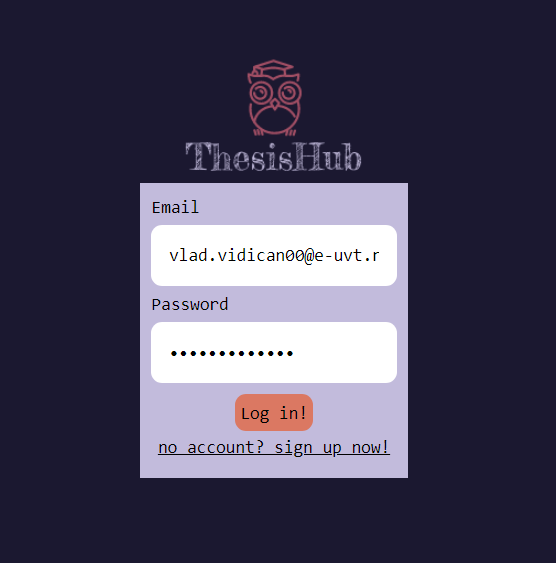
\includegraphics[scale=0.5]{images/LoginForm.PNG}
    \caption{Interfata autentificare}
\end{figure}
Dupa o autentificare reusita utilizatorul este redirectat catre pagina principala, 
de aici utilizatorul poate sa navigheze printre propunerile active de pe platforma.
Din motive de performanta am decis sa implementez paginare pentru cautarea de propuneri,
serverul este configurat sa returneze 4 elemente per pagina, in cazul in care nu toate propunerile sunt vizibile 
lista de propuneri permite scrolling, in partea de jos a pagini se afla interfata pentru navigarea printre paginile de propuneri. 

Utilizatorul are optiunea de a merge la pagina precedenta, pagina urmatoarea sau la oricare dintre cele vizibile, apasand 
pe unul dintre propuneri utilizator va fii redirectionat catre pagina acelei propuneri
\begin{figure}[H]
    \centering
    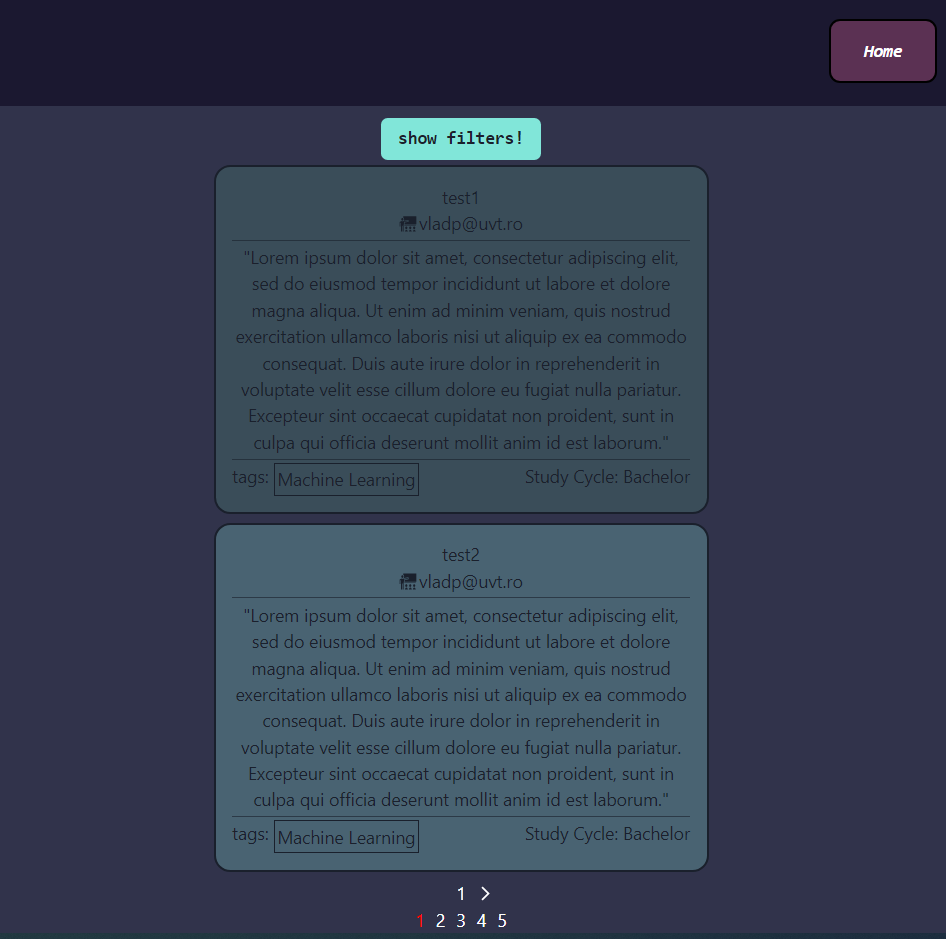
\includegraphics[scale=0.5]{images/HomePage.PNG}
    \caption{sistemul de navigare intre propuneri din pagina principala}
\end{figure}
Platforma suporta si cautarea filtrata dupa propuneri, apasand pe show filters utilizatorul poate sa filtreze propunerile 
in functie de urmatorii factori:
\begin{itemize}
    \item ciclu de studii pentru care este destinata propunerea.
    \item ce tip de cont a creat propunerea(student sau professor).
    \item anumite cuvinte cheie din titlul propunerii.
    \item anumite cuvinte chesie din descrierea propunerii.
    \item etichetele in care se incadreaza propunerile.
    aici utilizatorul poate sa aleaga si care sa fie relatia intre etichetele alese (sa contina cel putin una sau pe toate)
    daca sunt mai multe.
\end{itemize}
    Dupa ce utilizatorul alege toate filtrele de care este interesat poate apasa pe "Apply filters" pentru a reimprospata pagina
    doar cu propunerile ce respecta noile filtre, sau poate sa apese la orice moment pe "reset filters" pentru a debifa toate filtrele adaugate
\begin{figure}[H]
    \centering
    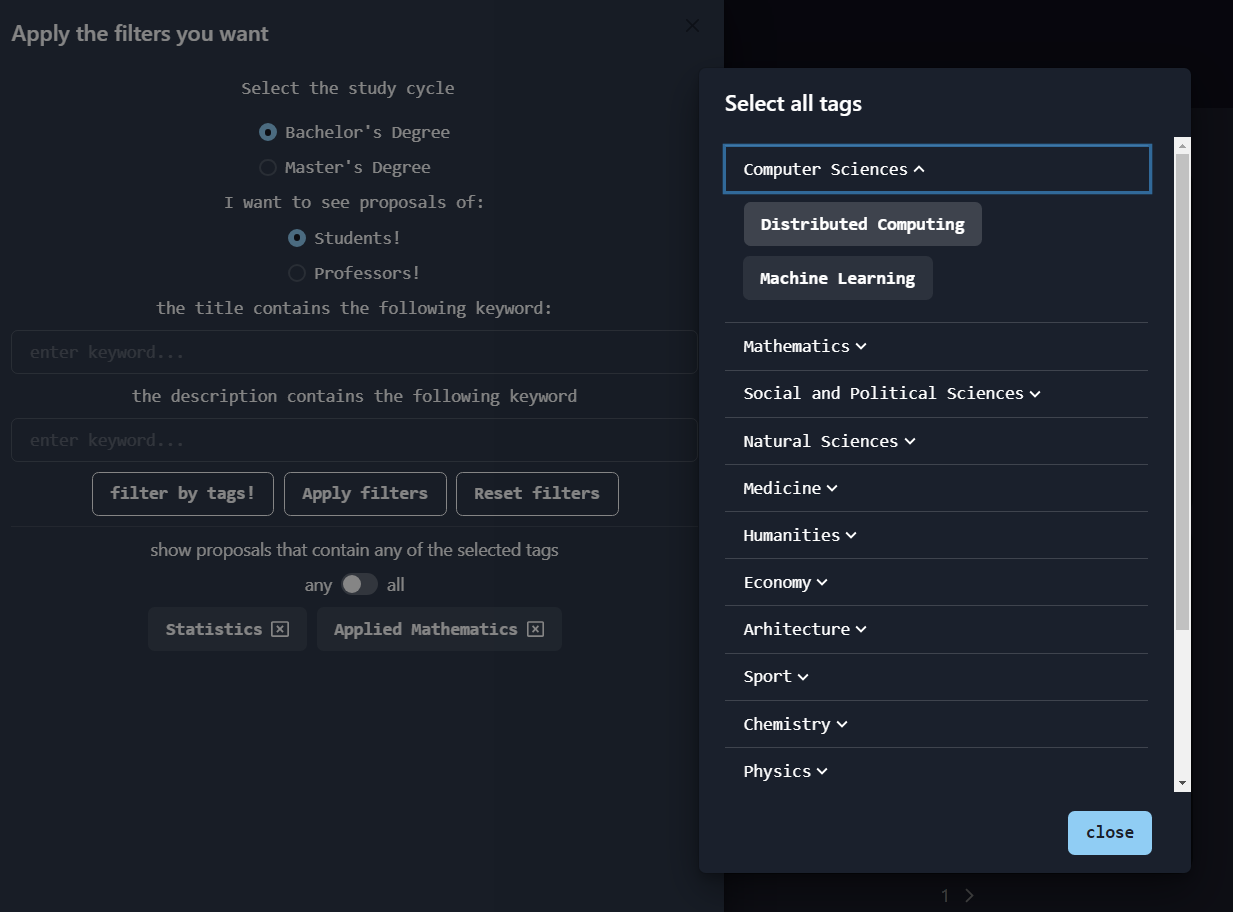
\includegraphics[scale=0.5]{images/advancedSearch.PNG}
    \caption{sistemul de cautare avanssata}
\end{figure}
Apasand pe una dintre propuneri, utilizatorul va fii dus catre pagina ei, aici are access la mai multe informatii despre aceasta propunere, cum ar fii:
\begin{itemize}
    \item Lista de Atasamente.
    \item Lista de comentarii.
    \item Aplicatiile curente pe aceasta tema.
\end{itemize}
si de aici acesta poate sa:
\begin{itemize}
    \item Adauge un comentariu nou.
    \item sa aplice pentru aceasta propunere.
    \item sa accepte una dintre aplicatii daca este detinatorul propunerii.
\end{itemize}
\begin{figure}[H]
    \centering
    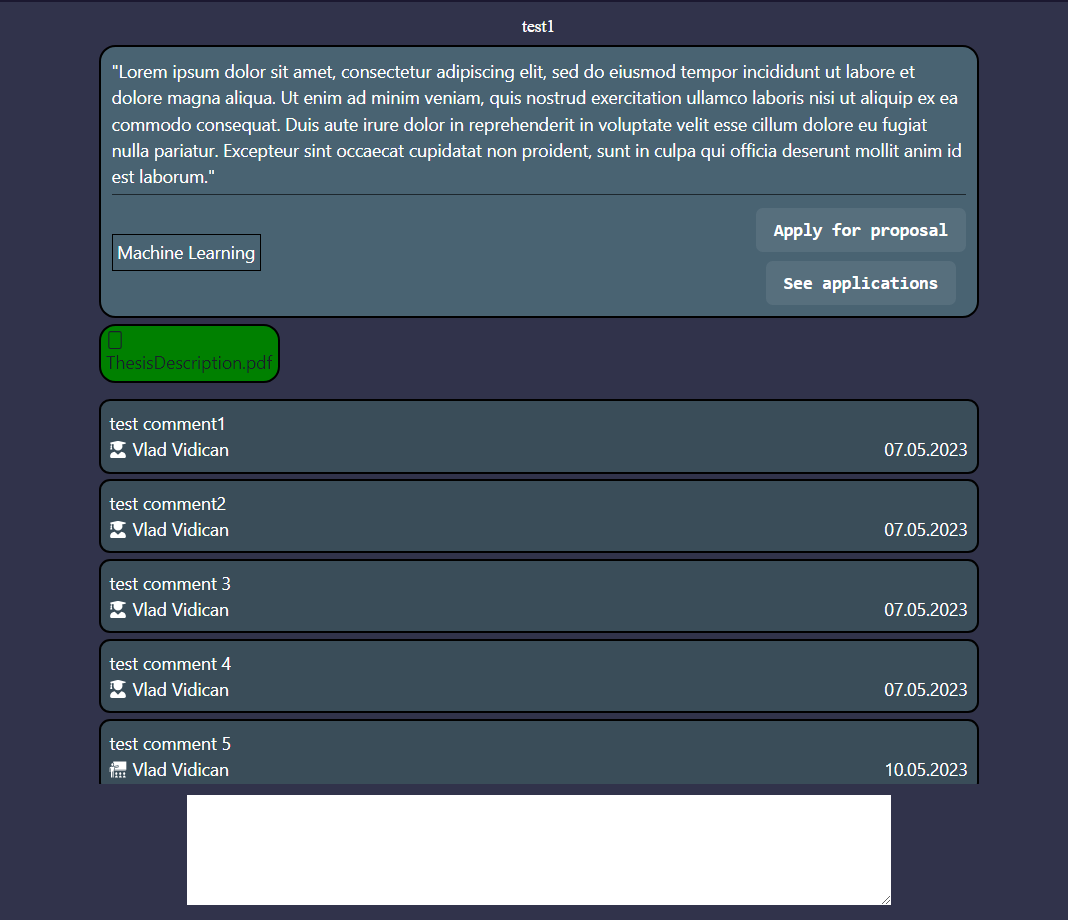
\includegraphics[scale=0.4]{images/ProposalPage.PNG}
    \caption{pagina de cautare google}
\end{figure}
\begin{figure}[H]
    \centering
    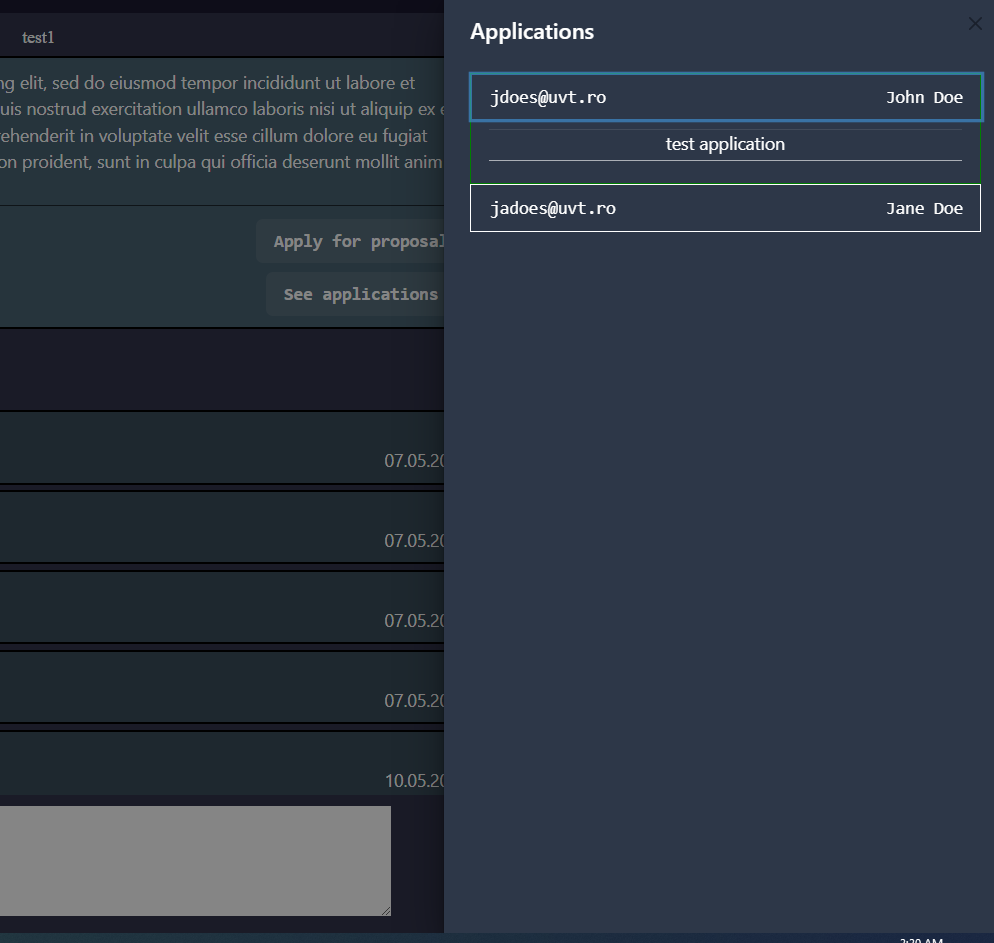
\includegraphics[scale=0.4]{images/Application.PNG}
    \caption{exemplu lista de aplicatii a unei propuneri}
\end{figure}
Utilizatorul poate sa isi creeze propria lui propunere apasand butonul "Create proposal" din bara de navigare
mai apoi acesta trebuie sa completeze urmatoarele campuri:
\begin{itemize}
    \item Titlul propunerii.
    \item Descrierea propunerii
    \item Atasamente (optional)
    \item sa aleaga cel putin o eticheta din cele disponibile
\end{itemize}
pentru a atasa etichete propunerii utilizatorul trebuie sa aleaga mai intai o categorie din bara din dreapta a pagini 
si din categoria alesa poate sa asocieze etichetele disponibile, utilizatorul nu este insa limitat la o singura categorie
\begin{figure}[H]
    \centering
    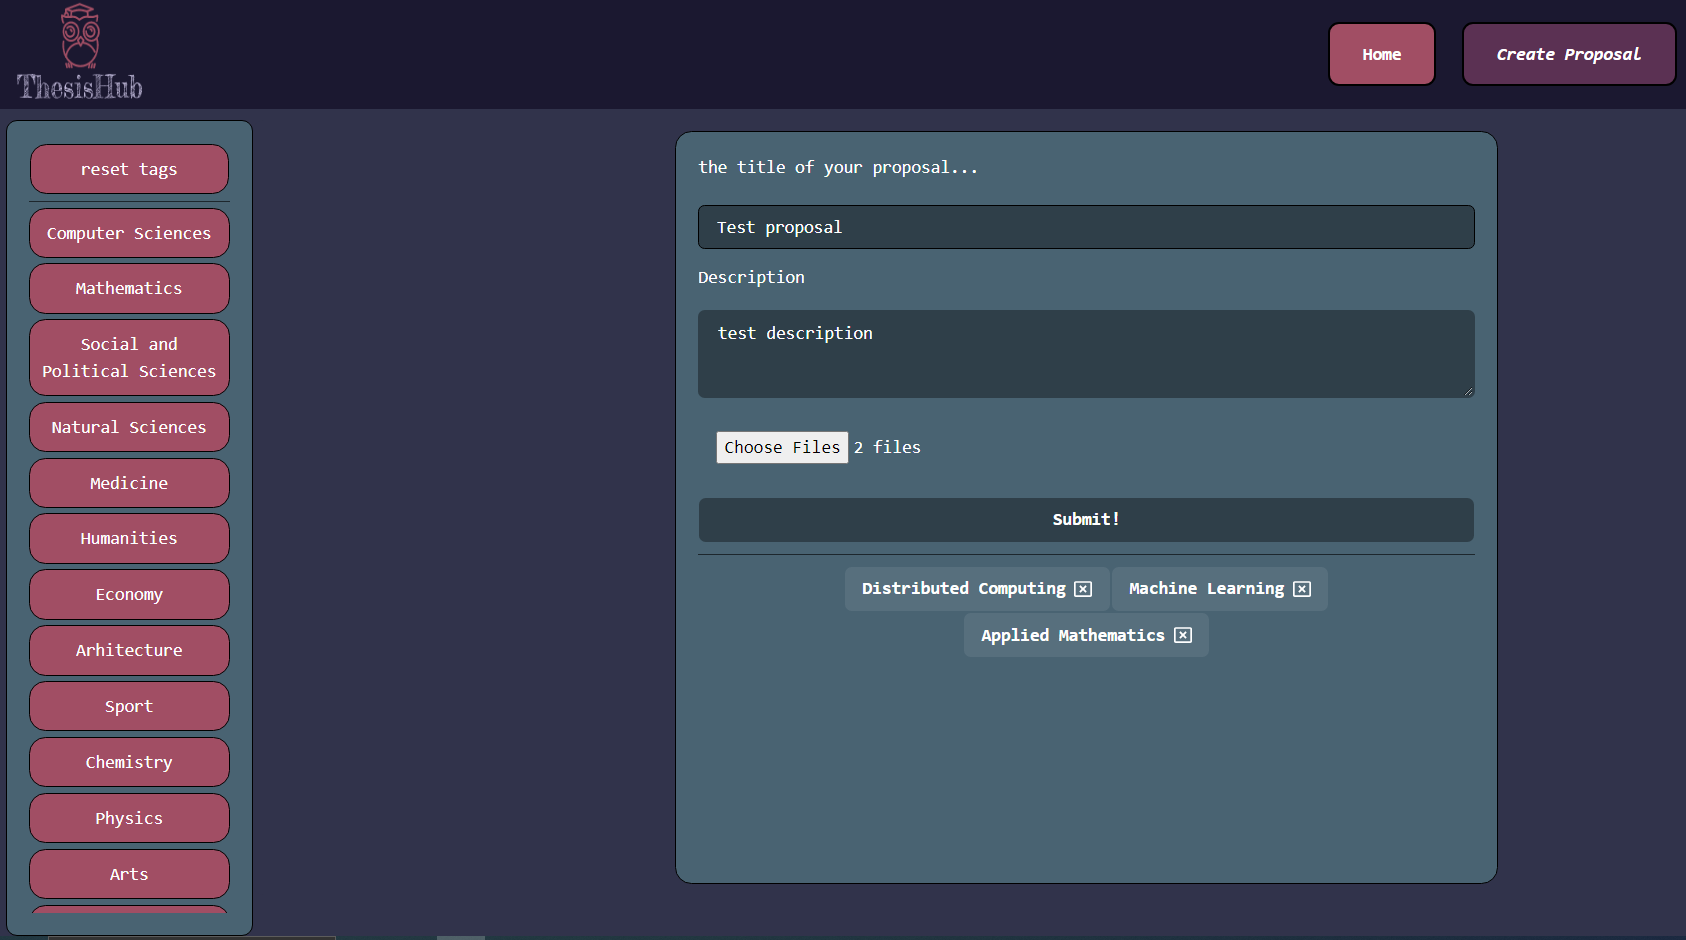
\includegraphics[scale=0.4]{images/CreateProposalPage.PNG}
    \caption{pagina pentru crearea propunerilor noi}
\end{figure}
\begin{figure}[H]
    \centering
    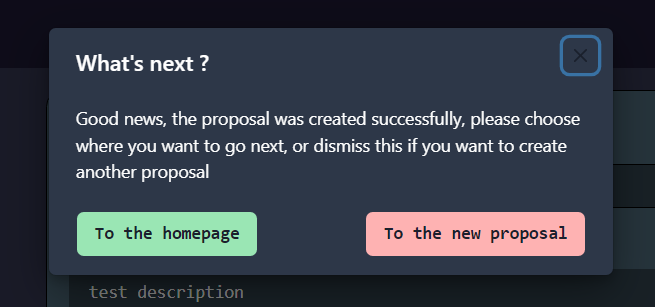
\includegraphics[scale=0.7]{images/ProposalCreated.PNG}
    \caption{Propunere creata cu success}
\end{figure}
Pentru a putea accessa pagina de mesagerie utilizatorul trebuie sa apese butonul "Conversations" din bara de navigare.

Odata ajuns pe pagina de mesagerie utilizatorul poate sa aleaga una dintre conversatiile actuale
apasand pe aceasta din bara laterala, sau poate sa apese "Add Users" pentru a initia conversatii noi.
Daca utilizatorul doreste sa initieze conversatii noi acessta trebuie doar sa introduca adresa de email
a acelei persoane in campul pentru cautarea a utilizatorilor, important de mentionat este ca nu este necesar
ca utilizatorii sa cunoasca adresa de email in totalitate a persoanelor cu care doresc sa initieze o conversatie, 
sistemul oferind sugestii in functie de literele introduse.

\begin{figure}[H]
    \centering
    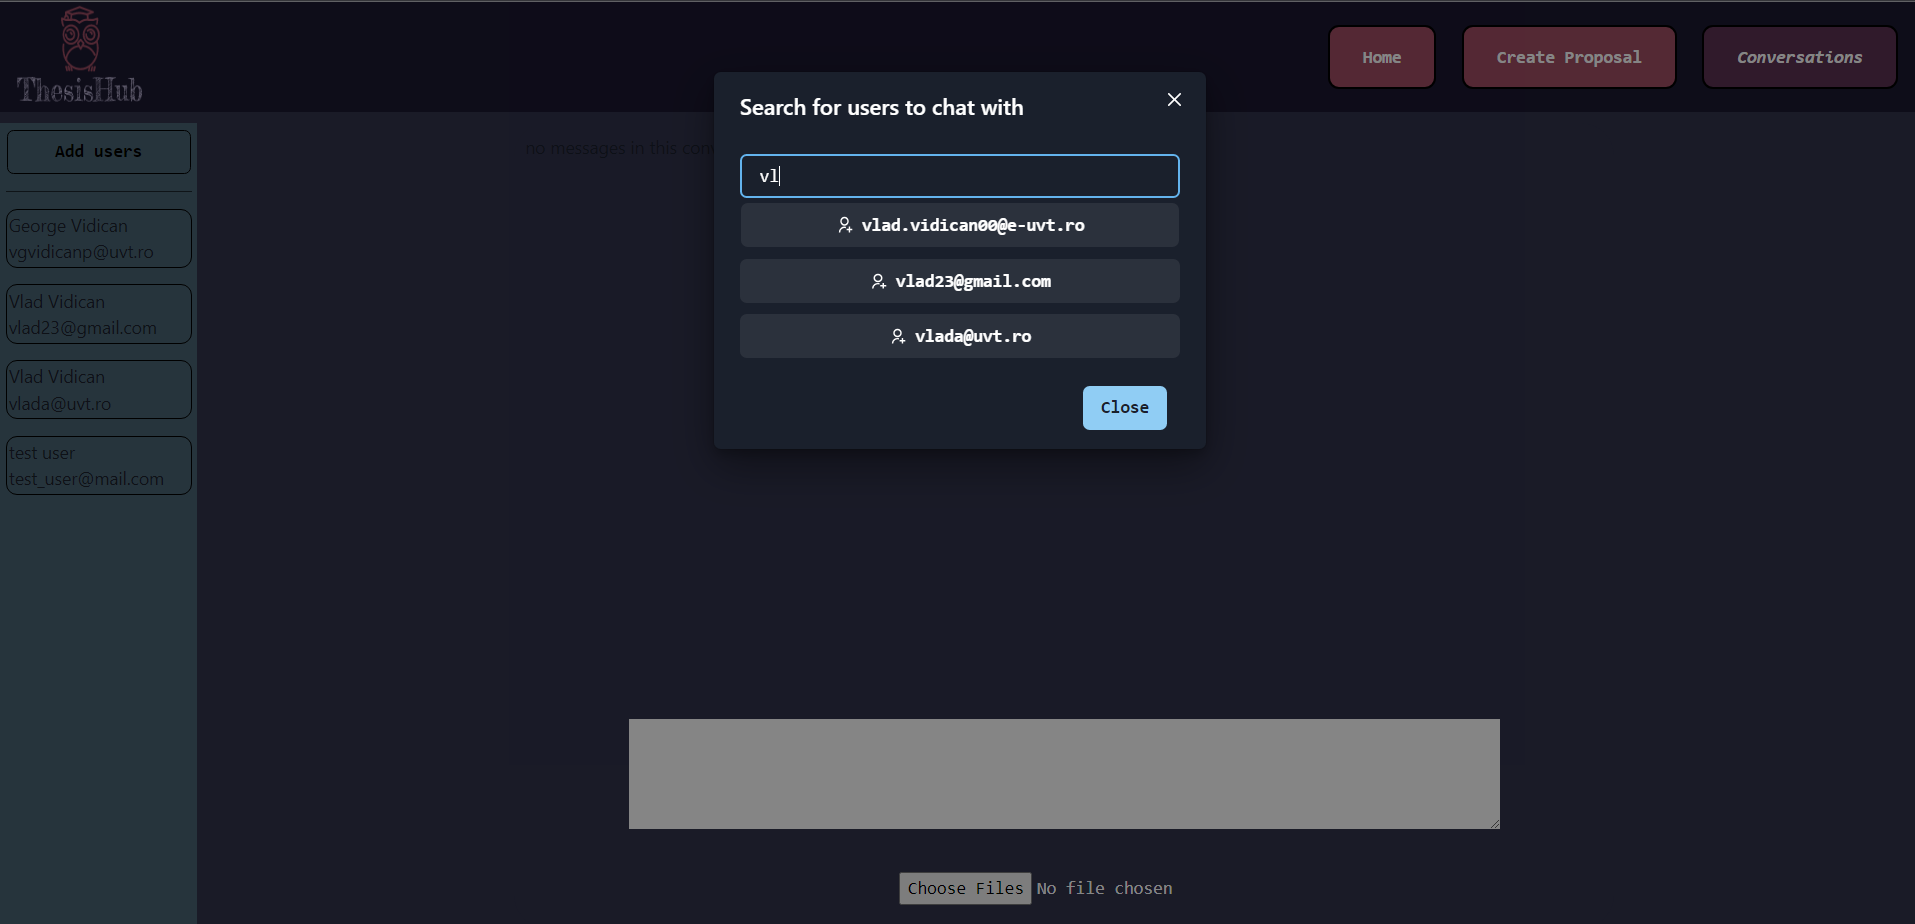
\includegraphics[scale=0.3]{images/AddUser.PNG}
    \caption{Interfata de initiere a unei conversatie}
\end{figure}
Odata cu alegerea unei conversatii utilizatorii pot trimite mesaje, acest lucru se poate face  
introducand textul dorit in zona de mesaje si apasand tasta ENTER,  
sistemul suporta si mesaje ce se intind pe mai multe linii, utilizatorul poate sa inceapa o linie noua apasand tastele SHIFT + ENTER
. Sistemul suporta de asemenea si trimiterea de fisiere, acestea sunt legate de mesaje, utilizatorul trebuie astfel doar sa aleaga
fisierele dorite si acestea vor fii trimise automat cu urmatorul mesaj.
\begin{figure}[H]
    \centering
    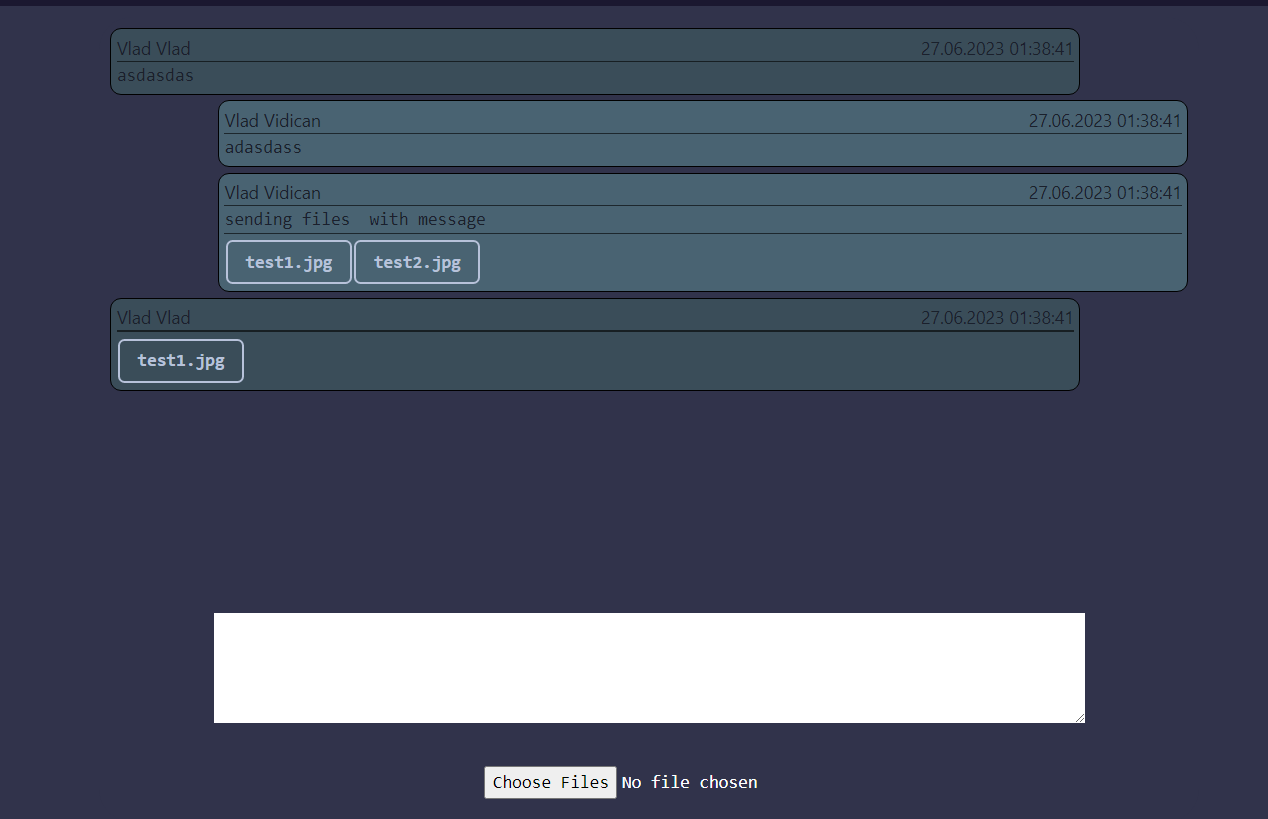
\includegraphics[scale=0.3]{images/SendMessages.PNG}
    \caption{Interfata Mesagerie}
\end{figure}
Administratorii au de asemenea posibilitatea de a accesa bordul de gestiune din bara de navigare(dashboard), 
aici pot vedea toate cerererile de inregistrare active de pe platforma, pe langa datele contului 
administatorii pot si sa revizuie dovezile de identitate atasate cererilor de inregistrare,
in cazul in care administratorul decide sa respinga o cerere atunci acesta este nevoit sa ii ofere utilizatorului si o justificare 
pentru decizia luata, un email de informare fiind trimis utilizatorului ulterior.
\begin{figure}[H]
    \centering
    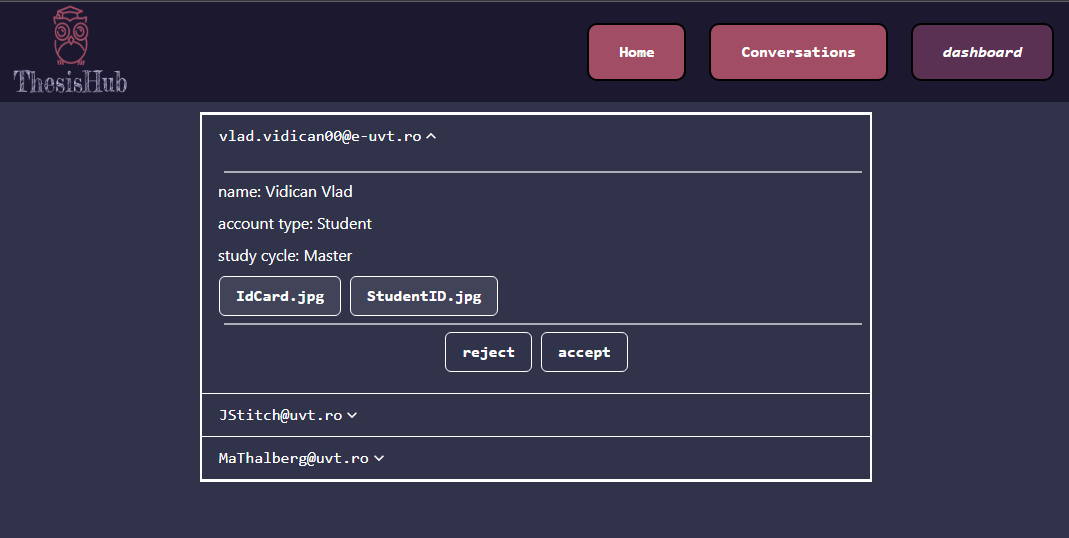
\includegraphics[scale=0.5]{images/Dashboard.PNG}
    \caption{Bordul de gestiune a administratorilor}
\end{figure}
\begin{figure}[H]
    \centering
    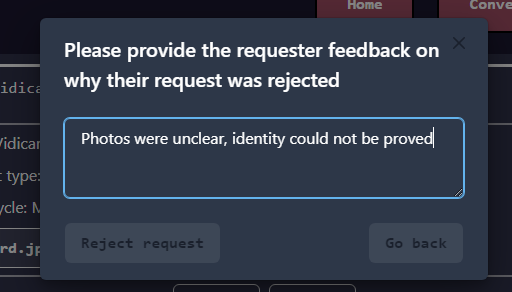
\includegraphics[scale=0.7]{images/RejectRequest.PNG}
    \caption{Exemplu respingerere cerere de inregistrare}
\end{figure}
\chapter{Concluzii si directii viitoare}
\section{directii viitoare}
Desi aplicatia in starea ei actuala ofera functionalitatile propuse aceasta are inca 
potential de dezvoltare, spre exemplu trecerea spre un sistem care sa suporte mai multe universtati. 
Desi in momentul de fata accesul nu este restrictionat efectiv unei singure institutii
sistemul nu suporta in starea sa actuala separarea logica a entitatilor in functie de universitateaa de apartenentă.
Aceasta functionalitate este insa necesara pentru a putea fii extinsa, fara aceasta administratorii unei universitati ar avea drepturi elevate
in ceea ce priveste gestionarea utilizatorilor asupra tuturor celorlalte universitati integrate in sistem.

Pentru a obtine acest rezultat un prim plan ar fii adaugarea unei colectii de universitati si modificarea schemei colectiilor: 
user, userTemp si proposal pentru a avea si o referinta catre o universitate, ar mai fii de asemenea nevoie de trecerea la un sistem
cu doua tipuri de administratori:
\begin{itemize}
    \item Administratori locali: acestia vor avea dreptul de a gestiona utilizatorii din aceeasi universitate ca si ei insasi
    \item Administratori ai aplicatiei: acestia nu apartin unei universitati anume si vor fii responsabili de adaugarea de 
    universitati, categorii si etichete noi in sistem, acestia nu se vor ocupa de gestionarea utilizatorilor in general exceptii fiind 
    adaugarea administratorului initial al unei universitati si adaugarea altor administratori de acest tip
\end{itemize}

O alta oportunitate de dezvoltare ar fii implementarea unei aplicatii mobile, dat fiind faptul ca serverul de backend 
este separat de logica generarii de pagini html si livrarii de continut static acesta ar putea fii integrat cu un client
de tip mobile fara a necesita nici o schimbare.

Posibilitatea de a folosi react native pentru dezvoltarea aplicatiei mobile este de asemenea un factor important deoareece
ar rezulta intr-o portare mai usoara, desi codul nu poate fii mapat unu la unu intre react si react native, aceste tehnologii folosind 
in spate elemente primitive diferite, acestea au insa un grad de similitudine ridicat
%\bibliography{mybib}
%\bibliographystyle{alpha}
%\addcontentsline{toc}{chapter}{Bibliography}
\end{document}
